% ----------------------------------------------------------------------
%
%                            TFMTesis.tex
%
%----------------------------------------------------------------------
%
% Este fichero contiene el "documento maestro" del documento. Lo único
% que hace es configurar el entorno LaTeX e incluir los ficheros .tex
% que contienen cada sección.
%
%----------------------------------------------------------------------
%
% Los ficheros necesarios para este documento son:
%
%       TeXiS/* : ficheros de la plantilla TeXiS.
%       Cascaras/* : ficheros con las partes del documento que no
%          son capítulos ni apéndices (portada, agradecimientos, etc.)
%       Capitulos/*.tex : capítulos de la tesis
%       Apendices/*.tex: apéndices de la tesis
%       constantes.tex: constantes LaTeX
%       config.tex : configuración de la "compilación" del documento
%       guionado.tex : palabras con guiones
%
% Para la bibliografía, además, se necesitan:
%
%       *.bib : ficheros con la información de las referencias
%
% ---------------------------------------------------------------------

\documentclass[12pt,a4paper,twoside]{book}

%
% Definimos  el   comando  \compilaCapitulo,  que   luego  se  utiliza
% (opcionalmente) en config.tex. Quedaría  mejor si también se definiera
% en  ese fichero,  pero por  el modo  en el  que funciona  eso  no es
% posible. Puedes consultar la documentación de ese fichero para tener
% más  información. Definimos también  \compilaApendice, que  tiene el
% mismo  cometido, pero  que se  utiliza para  compilar  únicamente un
% apéndice.
%
%
% Si  queremos   compilar  solo   una  parte  del   documento  podemos
% especificar mediante  \includeonly{...} qué ficheros  son los únicos
% que queremos  que se incluyan.  Esto  es útil por  ejemplo para sólo
% compilar un capítulo.
%
% El problema es que todos aquellos  ficheros que NO estén en la lista
% NO   se  incluirán...  y   eso  también   afecta  a   ficheros  de
% la plantilla...
%
% Total,  que definimos  una constante  con los  ficheros  que siempre
% vamos a querer compilar  (aquellos relacionados con configuración) y
% luego definimos \compilaCapitulo.
\newcommand{\ficherosBasicosTeXiS}{%
TeXiS/TeXiS_pream,TeXiS/TeXiS_cab,TeXiS/TeXiS_bib,TeXiS/TeXiS_cover%
}
\newcommand{\ficherosBasicosTexto}{%
constantes,guionado,Cascaras/bibliografia,config%
}
\newcommand{\compilaCapitulo}[1]{%
\includeonly{\ficherosBasicosTeXiS,\ficherosBasicosTexto,Capitulos/#1}%
}

\newcommand{\compilaApendice}[1]{%
\includeonly{\ficherosBasicosTeXiS,\ficherosBasicosTexto,Apendices/#1}%
}

% #1 = tikz options (optional)
% #2 = total width (e.g. 7cm)
% #3 = height      (e.g. 0.5cm)
% #4 = wins
% #5 = draws
% #6 = losses
\newcommand{\ResultBar}[6][]{%
  \begingroup
  % compute totals & scaled lengths
  \pgfmathsetmacro{\TotalGames}{#4 + #5 + #6}%
  \pgfmathsetlengthmacro{\TotalWidth}{#2}%
  \pgfmathsetlengthmacro{\BarHeight}{#3}%
  \pgfmathsetlengthmacro{\WinWidth}{#4/\TotalGames*\TotalWidth}%
  \pgfmathsetlengthmacro{\DrawWidth}{#5/\TotalGames*\TotalWidth}%
  \pgfmathsetlengthmacro{\LossWidth}{#6/\TotalGames*\TotalWidth}%
  %
  \begin{tikzpicture}[#1]
    % coloured segments
    \fill[green!70!black] (0,0) rectangle (\WinWidth,\BarHeight);
    \fill[gray] (\WinWidth,0) rectangle (\WinWidth+\DrawWidth,\BarHeight);
    \fill[red!70!black] (\WinWidth+\DrawWidth,0)
                       rectangle (\WinWidth+\DrawWidth+\LossWidth,\BarHeight);
    % outer border
    \draw (0,0) rectangle (\TotalWidth,\BarHeight);
    % labels above each segment
    % conditional labels
    \ifnum#4>0
      \node[font=\footnotesize] at (\WinWidth/2,1.4*\BarHeight)
        {\textbf{#4} wins};
    \fi
    \ifnum#5>0
      \node[font=\footnotesize] at (\WinWidth + \DrawWidth/2,1.4*\BarHeight)
        {\textbf{#5} draws};
    \fi
    \ifnum#6>0
      \node[font=\footnotesize] at (\WinWidth+\DrawWidth + \LossWidth/2,1.4*\BarHeight)
        {\textbf{#6} losses};
    \fi
  \end{tikzpicture}%
  \endgroup
}

%- - - - - - - - - - - - - - - - - - - - - - - - - - - - - - - - - - -
%            Preámbulo del documento. Configuraciones varias
%- - - - - - - - - - - - - - - - - - - - - - - - - - - - - - - - - - -

% Define  el  tipo  de  compilación que  estamos  haciendo.   Contiene
% definiciones  de  constantes que  cambian  el  comportamiento de  la
% compilación. Debe incluirse antes del paquete TeXiS/TeXiS.sty
%---------------------------------------------------------------------
%
%                          config.tex
%
%---------------------------------------------------------------------
%
% Contiene la  definición de constantes  que determinan el modo  en el
% que se compilará el documento.
%
%---------------------------------------------------------------------
%
% En concreto, podemos  indicar si queremos "modo release",  en el que
% no  aparecerán  los  comentarios  (creados  mediante  \com{Texto}  o
% \comp{Texto}) ni los "por  hacer" (creados mediante \todo{Texto}), y
% sí aparecerán los índices. El modo "debug" (o mejor dicho en modo no
% "release" muestra los índices  (construirlos lleva tiempo y son poco
% útiles  salvo  para   la  versión  final),  pero  sí   el  resto  de
% anotaciones.
%
% Si se compila con LaTeX (no  con pdflatex) en modo Debug, también se
% muestran en una esquina de cada página las entradas (en el índice de
% palabras) que referencian  a dicha página (consulta TeXiS_pream.tex,
% en la parte referente a show).
%
% El soporte para  el índice de palabras en  TeXiS es embrionario, por
% lo  que no  asumas que  esto funcionará  correctamente.  Consulta la
% documentación al respecto en TeXiS_pream.tex.
%
%
% También  aquí configuramos  si queremos  o  no que  se incluyan  los
% acrónimos  en el  documento final  en la  versión release.  Para eso
% define (o no) la constante \acronimosEnRelease.
%
% Utilizando \compilaCapitulo{nombre}  podemos también especificar qué
% capítulo(s) queremos que se compilen. Si no se pone nada, se compila
% el documento  completo.  Si se pone, por  ejemplo, 01Introduccion se
% compilará únicamente el fichero Capitulos/01Introduccion.tex
%
% Para compilar varios  capítulos, se separan sus nombres  con comas y
% no se ponen espacios de separación.
%
% En realidad  la macro \compilaCapitulo  está definida en  el fichero
% principal tesis.tex.
%
%---------------------------------------------------------------------


% Comentar la línea si no se compila en modo release.
% TeXiS hará el resto.
% ¡¡¡Si cambias esto, haz un make clean antes de recompilar!!!
\def\release{1}


% Descomentar la linea si se quieren incluir los
% acrónimos en modo release (en modo debug
% no se incluirán nunca).
% ¡¡¡Si cambias esto, haz un make clean antes de recompilar!!!
%\def\acronimosEnRelease{1}


% Descomentar la línea para establecer el capítulo que queremos
% compilar

% \compilaCapitulo{01Introduccion}
% \compilaCapitulo{02EstructuraYGeneracion}
% \compilaCapitulo{03Edicion}
% \compilaCapitulo{04Imagenes}
% \compilaCapitulo{05Bibliografia}
% \compilaCapitulo{06Makefile}

% \compilaApendice{01AsiSeHizo}

% Variable local para emacs, para  que encuentre el fichero maestro de
% compilación y funcionen mejor algunas teclas rápidas de AucTeX
%%%
%%% Local Variables:
%%% mode: latex
%%% TeX-master: "./Tesis.tex"
%%% End:


% Paquete de la plantilla
\usepackage{TeXiS/TeXiS}

% Incluimos el fichero con comandos de constantes
%---------------------------------------------------------------------
%
%                          constantes.tex
%
%---------------------------------------------------------------------
%
% Fichero que  declara nuevos comandos LaTeX  sencillos realizados por
% comodidad en la escritura de determinadas palabras
%
%---------------------------------------------------------------------

%%%%%%%%%%%%%%%%%%%%%%%%%%%%%%%%%%%%%%%%%%%%%%%%%%%%%%%%%%%%%%%%%%%%%%
% Comando: 
%
%       \titulo
%
% Resultado: 
%
% Escribe el título del documento.
%%%%%%%%%%%%%%%%%%%%%%%%%%%%%%%%%%%%%%%%%%%%%%%%%%%%%%%%%%%%%%%%%%%%%%
\def\titulo{AlphaDeepChess: chess engine based on alpha-beta pruning}

%%%%%%%%%%%%%%%%%%%%%%%%%%%%%%%%%%%%%%%%%%%%%%%%%%%%%%%%%%%%%%%%%%%%%%
% Comando: 
%
%       \autor
%
% Resultado: 
%
% Escribe el autor del documento.
%%%%%%%%%%%%%%%%%%%%%%%%%%%%%%%%%%%%%%%%%%%%%%%%%%%%%%%%%%%%%%%%%%%%%%
\def\autor{Juan Girón Herranz y Yi Wang Qiu}

% Variable local para emacs, para  que encuentre el fichero maestro de
% compilación y funcionen mejor algunas teclas rápidas de AucTeX

%%%
%%% Local Variables:
%%% mode: latex
%%% TeX-master: "tesis.tex"
%%% End:


% Sacamos en el log de la compilación el copyright
%\typeout{Copyright Marco Antonio and Pedro Pablo Gomez Martin}

%
% "Metadatos" para el PDF
%
\ifpdf\hypersetup{%
    pdftitle = {\titulo},
    pdfsubject = {Plantilla de Tesis},
    pdfkeywords = {Plantilla, LaTeX, tesis, trabajo de
      investigación, trabajo de Master},
    pdfauthor = {\textcopyright\ \autor},
    pdfcreator = {\LaTeX\ con el paquete \flqq hyperref\frqq},
    pdfproducer = {pdfeTeX-0.\the\pdftexversion\pdftexrevision},
    }
    \pdfinfo{/CreationDate (\today)}
\fi


%- - - - - - - - - - - - - - - - - - - - - - - - - - - - - - - - - - -
%                        Documento
%- - - - - - - - - - - - - - - - - - - - - - - - - - - - - - - - - - -
\makeindex
\setlength{\parindent}{0pt} % Eliminar sangría

\begin{document}

% Incluimos el  fichero de definición de guionado  de algunas palabras
% que LaTeX no ha dividido como debería
%----------------------------------------------------------------
%
%                          guionado.tex
%
%----------------------------------------------------------------
%
% Fichero con algunas divisiones de palabras que LaTeX no
% hace correctamente si no se le da alguna ayuda.
%
%----------------------------------------------------------------

\hyphenation{
% a
abs-trac-to
abs-trac-tos
abs-trac-ta
abs-trac-tas
ac-tua-do-res
a-gra-de-ci-mien-tos
ana-li-za-dor
an-te-rio-res
an-te-rior-men-te
apa-rien-cia
a-pro-pia-do
a-pro-pia-dos
a-pro-pia-da
a-pro-pia-das
a-pro-ve-cha-mien-to
a-que-llo
a-que-llos
a-que-lla
a-que-llas
a-sig-na-tu-ra
a-sig-na-tu-ras
a-so-cia-da
a-so-cia-das
a-so-cia-do
a-so-cia-dos
au-to-ma-ti-za-do
% b
batch
bi-blio-gra-fía
bi-blio-grá-fi-cas
bien
bo-rra-dor
boo-l-ean-expr
% c
ca-be-ce-ra
call-me-thod-ins-truc-tion
cas-te-lla-no
cir-cuns-tan-cia
cir-cuns-tan-cias
co-he-ren-te
co-he-ren-tes
co-he-ren-cia
co-li-bri
co-men-ta-rio
co-mer-cia-les
co-no-ci-mien-to
cons-cien-te
con-si-de-ra-ba
con-si-de-ra-mos
con-si-de-rar-se
cons-tan-te
cons-trucción
cons-tru-ye
cons-tru-ir-se
con-tro-le
co-rrec-ta-men-te
co-rres-pon-den
co-rres-pon-dien-te
co-rres-pon-dien-tes
co-ti-dia-na
co-ti-dia-no
crean
cris-ta-li-zan
cu-rri-cu-la
cu-rri-cu-lum
cu-rri-cu-lar
cu-rri-cu-la-res
% d
de-di-ca-do
de-di-ca-dos
de-di-ca-da
de-di-ca-das
de-rro-te-ro
de-rro-te-ros
de-sa-rro-llo
de-sa-rro-llos
de-sa-rro-lla-do
de-sa-rro-lla-dos
de-sa-rro-lla-da
de-sa-rro-lla-das
de-sa-rro-lla-dor
de-sa-rro-llar
des-cri-bi-re-mos
des-crip-ción
des-crip-cio-nes
des-cri-to
des-pués
de-ta-lla-do
de-ta-lla-dos
de-ta-lla-da
de-ta-lla-das
di-a-gra-ma
di-a-gra-mas
di-se-ños
dis-po-ner
dis-po-ni-bi-li-dad
do-cu-men-ta-da
do-cu-men-to
do-cu-men-tos
% e
edi-ta-do
e-du-ca-ti-vo
e-du-ca-ti-vos
e-du-ca-ti-va
e-du-ca-ti-vas
e-la-bo-ra-do
e-la-bo-ra-dos
e-la-bo-ra-da
e-la-bo-ra-das
es-co-llo
es-co-llos
es-tu-dia-do
es-tu-dia-dos
es-tu-dia-da
es-tu-dia-das
es-tu-dian-te
e-va-lua-cio-nes
e-va-lua-do-res
exis-ten-tes
exhaus-ti-va
ex-pe-rien-cia
ex-pe-rien-cias
% f
for-ma-li-za-do
% g
ge-ne-ra-ción
ge-ne-ra-dor
ge-ne-ra-do-res
ge-ne-ran
% h
he-rra-mien-ta
he-rra-mien-tas
% i
i-dio-ma
i-dio-mas
im-pres-cin-di-ble
im-pres-cin-di-bles
in-de-xa-do
in-de-xa-dos
in-de-xa-da
in-de-xa-das
in-di-vi-dual
in-fe-ren-cia
in-fe-ren-cias
in-for-ma-ti-ca
in-gre-dien-te
in-gre-dien-tes
in-me-dia-ta-men-te
ins-ta-la-do
ins-tan-cias
% j
% k
% l
len-gua-je
li-be-ra-to-rio
li-be-ra-to-rios
li-be-ra-to-ria
li-be-ra-to-rias
li-mi-ta-do
li-te-ra-rio
li-te-ra-rios
li-te-ra-ria
li-te-ra-rias
lo-tes
% m
ma-ne-ra
ma-nual
mas-que-ra-de
ma-yor
me-mo-ria
mi-nis-te-rio
mi-nis-te-rios
mo-de-lo
mo-de-los
mo-de-la-do
mo-du-la-ri-dad
mo-vi-mien-to
% n
na-tu-ral
ni-vel
nues-tro
% o
obs-tan-te
o-rien-ta-do
o-rien-ta-dos
o-rien-ta-da
o-rien-ta-das
% p
pa-ra-le-lo
pa-ra-le-la
par-ti-cu-lar
par-ti-cu-lar-men-te
pe-da-gó-gi-ca
pe-da-gó-gi-cas
pe-da-gó-gi-co
pe-da-gó-gi-cos
pe-rio-di-ci-dad
per-so-na-je
plan-te-a-mien-to
plan-te-a-mien-tos
po-si-ción
pre-fe-ren-cia
pre-fe-ren-cias
pres-cin-di-ble
pres-cin-di-bles
pri-me-ra
pro-ble-ma
pro-ble-mas
pró-xi-mo
pu-bli-ca-cio-nes
pu-bli-ca-do
% q
% r
rá-pi-da
rá-pi-do
ra-zo-na-mien-to
ra-zo-na-mien-tos
re-a-li-zan-do
re-fe-ren-cia
re-fe-ren-cias
re-fe-ren-cia-da
re-fe-ren-cian
re-le-van-tes
re-pre-sen-ta-do
re-pre-sen-ta-dos
re-pre-sen-ta-da
re-pre-sen-ta-das
re-pre-sen-tar-lo
re-qui-si-to
re-qui-si-tos
res-pon-der
res-pon-sa-ble
% s
se-pa-ra-do
si-guien-do
si-guien-te
si-guien-tes
si-guie-ron
si-mi-lar
si-mi-la-res
si-tua-ción
% t
tem-pe-ra-ments
te-ner
trans-fe-ren-cia
trans-fe-ren-cias
% u
u-sua-rio
Unreal-Ed
% v
va-lor
va-lo-res
va-rian-te
ver-da-de-ro
ver-da-de-ros
ver-da-de-ra
ver-da-de-ras
ver-da-de-ra-men-te
ve-ri-fi-ca
% w
% x
% y
% z
}
% Variable local para emacs, para que encuentre el fichero
% maestro de compilación
%%%
%%% Local Variables:
%%% mode: latex
%%% TeX-master: "./Tesis.tex"
%%% End:


% Marcamos  el inicio  del  documento para  la  numeración de  páginas
% (usando números romanos para esta primera fase).
\frontmatter
\pagestyle{empty}

%---------------------------------------------------------------------
%
%                          configCover.tex
%
%---------------------------------------------------------------------
%
% cover.tex
% Copyright 2009 Marco Antonio Gomez-Martin, Pedro Pablo Gomez-Martin
%
% This file belongs to the TeXiS manual, a LaTeX template for writting
% Thesis and other documents. The complete last TeXiS package can
% be obtained from http://gaia.fdi.ucm.es/projects/texis/
%
% Although the TeXiS template itself is distributed under the 
% conditions of the LaTeX Project Public License
% (http://www.latex-project.org/lppl.txt), the manual content
% uses the CC-BY-SA license that stays that you are free:
%
%    - to share & to copy, distribute and transmit the work
%    - to remix and to adapt the work
%
% under the following conditions:
%
%    - Attribution: you must attribute the work in the manner
%      specified by the author or licensor (but not in any way that
%      suggests that they endorse you or your use of the work).
%    - Share Alike: if you alter, transform, or build upon this
%      work, you may distribute the resulting work only under the
%      same, similar or a compatible license.
%
% The complete license is available in
% http://creativecommons.org/licenses/by-sa/3.0/legalcode
%
%---------------------------------------------------------------------
%
% Fichero que contiene la configuración de la portada y de la 
% primera hoja del documento.
%
%---------------------------------------------------------------------


% Pueden configurarse todos los elementos del contenido de la portada
% utilizando comandos.

%%%%%%%%%%%%%%%%%%%%%%%%%%%%%%%%%%%%%%%%%%%%%%%%%%%%%%%%%%%%%%%%%%%%%%
% Título del documento:
% \tituloPortada{titulo}
% Nota:
% Si no se define se utiliza el del \titulo. Este comando permite
% cambiar el título de forma que se especifiquen dónde se quieren
% los retornos de carro cuando se utilizan fuentes grandes.
%%%%%%%%%%%%%%%%%%%%%%%%%%%%%%%%%%%%%%%%%%%%%%%%%%%%%%%%%%%%%%%%%%%%%%
\tituloPortada{%
AlphaDeepChess: motor de ajedrez basado en podas alpha-beta
}


%%%%%%%%%%%%%%%%%%%%%%%%%%%%%%%%%%%%%%%%%%%%%%%%%%%%%%%%%%%%%%%%%%%%%%
% Título del documento en inglés:
% \tituloPortadaEng{titulo}
% Nota:
% Si no se define se utiliza el del \titulo. Este comando permite
% cambiar el título de forma que se especifiquen dónde se quieren
% los retornos de carro cuando se utilizan fuentes grandes.
%%%%%%%%%%%%%%%%%%%%%%%%%%%%%%%%%%%%%%%%%%%%%%%%%%%%%%%%%%%%%%%%%%%%%%
\tituloPortadaEng{%
AlphaDeepChess: chess engine based on alpha-beta pruning
}

%%%%%%%%%%%%%%%%%%%%%%%%%%%%%%%%%%%%%%%%%%%%%%%%%%%%%%%%%%%%%%%%%%%%%%
% Autor del documento:
% \autorPortada{Nombre}
% Se utiliza en la portada y en el valor por defecto del
% primer subtítulo de la segunda portada.
%%%%%%%%%%%%%%%%%%%%%%%%%%%%%%%%%%%%%%%%%%%%%%%%%%%%%%%%%%%%%%%%%%%%%%
\autorPortada{Juan Girón Herranz \\ Yi Wang Qiu}

%%%%%%%%%%%%%%%%%%%%%%%%%%%%%%%%%%%%%%%%%%%%%%%%%%%%%%%%%%%%%%%%%%%%%%
% Fecha de publicación:
% \fechaPublicacion{Fecha}
% Puede ser vacío. Aparece en la última línea de ambas portadas
%%%%%%%%%%%%%%%%%%%%%%%%%%%%%%%%%%%%%%%%%%%%%%%%%%%%%%%%%%%%%%%%%%%%%%
% Descomentar para que ponga siempre la fecha actual
\fechaPublicacion{\today}
%\fechaPublicacion{\textcolor{red}{DIA de MES de AÑO}}

%%%%%%%%%%%%%%%%%%%%%%%%%%%%%%%%%%%%%%%%%%%%%%%%%%%%%%%%%%%%%%%%%%%%%%
% Imagen de la portada (y escala)
% \imagenPortada{Fichero}
% \escalaImagenPortada{Numero}
% Si no se especifica, se utiliza la imagen TODO.pdf
%%%%%%%%%%%%%%%%%%%%%%%%%%%%%%%%%%%%%%%%%%%%%%%%%%%%%%%%%%%%%%%%%%%%%%
% imagen en blanco y negro
%\imagenPortada{Imagenes/Vectorial/escudoUCM}
%imagen en color
\imagenPortada{Imagenes/Bitmap/escudoUCMcolor}
\escalaImagenPortada{.2}

%%%%%%%%%%%%%%%%%%%%%%%%%%%%%%%%%%%%%%%%%%%%%%%%%%%%%%%%%%%%%%%%%%%%%%
% Tipo de documento.
% \tipoDocumento{Tipo}
% Para el texto justo debajo del escudo.
% Si no se indica, se utiliza "TESIS DOCTORAL".
%%%%%%%%%%%%%%%%%%%%%%%%%%%%%%%%%%%%%%%%%%%%%%%%%%%%%%%%%%%%%%%%%%%%%%
\tipoDocumento{Trabajo de Fin de Grado}
%\tipoDocumento{Final Degree Project}

%%%%%%%%%%%%%%%%%%%%%%%%%%%%%%%%%%%%%%%%%%%%%%%%%%%%%%%%%%%%%%%%%%%%%%
% Institución/departamento asociado al documento.
% \institucion{Nombre}
% Puede tener varias líneas. Se utiliza en las dos portadas.
% Si no se indica aparecerá vacío.
%%%%%%%%%%%%%%%%%%%%%%%%%%%%%%%%%%%%%%%%%%%%%%%%%%%%%%%%%%%%%%%%%%%%%%
\institucion{%
Grado en Ingeniería de Computadores\\[0.2em]
Grado en Desarrollo de Videojuegos\\[0.2em]
Facultad de Informática\\[0.2em]
Universidad Complutense de Madrid
%Bachelor's Degree in Computer Engineering\\[0.2em]
%Bachelor's Degree in Videogame Development\\[0.2em]
%Faculty of Computer Science\\[0.2em]
%Complutense University of Madrid
}

%%%%%%%%%%%%%%%%%%%%%%%%%%%%%%%%%%%%%%%%%%%%%%%%%%%%%%%%%%%%%%%%%%%%%%
% Director del trabajo.
% \directorPortada{Nombre}
% Se utiliza para el valor por defecto del segundo subtítulo, donde
% se indica quién es el director del trabajo.
% Si se fuerza un subtítulo distinto, no hace falta definirlo.
%%%%%%%%%%%%%%%%%%%%%%%%%%%%%%%%%%%%%%%%%%%%%%%%%%%%%%%%%%%%%%%%%%%%%%
\directorPortada{Ignacio Fábregas Alfaro\\Rubén Rafael Rubio Cuéllar}


%%%%%%%%%%%%%%%%%%%%%%%%%%%%%%%%%%%%%%%%%%%%%%%%%%%%%%%%%%%%%%%%%%%%%%
% Colaborador en la dirección del trabajo.
% \colaboradorPortada{Nombre}
% Se utiliza para el valor por defecto del segundo subtítulo, donde
% se indica quién es el colaborador en la dirección del trabajo.
% Si se fuerza un subtítulo distinto, no hace falta definirlo.
%%%%%%%%%%%%%%%%%%%%%%%%%%%%%%%%%%%%%%%%%%%%%%%%%%%%%%%%%%%%%%%%%%%%%%
%\colaboradorPortada{\textcolor{red}{Colaborador 1\\Colaborador 2}}


%%%%%%%%%%%%%%%%%%%%%%%%%%%%%%%%%%%%%%%%%%%%%%%%%%%%%%%%%%%%%%%%%%%%%%
% Texto del primer subtítulo de la segunda portada.
% \textoPrimerSubtituloPortada{Texto}
% Para configurar el primer "texto libre" de la segunda portada.
% Si no se especifica se indica "Memoria que presenta para optar al
% título de Doctor en Informática" seguido del \autorPortada.
%%%%%%%%%%%%%%%%%%%%%%%%%%%%%%%%%%%%%%%%%%%%%%%%%%%%%%%%%%%%%%%%%%%%%%
\textoPrimerSubtituloPortada{%
\textbf{Trabajo de Fin de Grado en Ingeniería de Computadores}\\ [0.3em]
\textbf{Trabajo de Fin de Grado en Desarrollo de Videojuegos}\\ [0.3em]
%\textbf{Final Degree Project in Computer Engineering}\\ [0.3em]
%\textbf{Final Degree Project in Videogame Development}\\ [0.3em]
}

%%%%%%%%%%%%%%%%%%%%%%%%%%%%%%%%%%%%%%%%%%%%%%%%%%%%%%%%%%%%%%%%%%%%%%
% Texto del segundo subtítulo de la segunda portada.
% \textoSegundoSubtituloPortada{Texto}
% Para configurar el segundo "texto libre" de la segunda portada.
% Si no se especifica se indica "Dirigida por el Doctor" seguido
% del \directorPortada.
%%%%%%%%%%%%%%%%%%%%%%%%%%%%%%%%%%%%%%%%%%%%%%%%%%%%%%%%%%%%%%%%%%%%%%
\textoSegundoSubtituloPortada{%
%\textbf{Convocation: }\textit{June \the\year}%\\[0.2em]
\textbf{Convocatoria: }\textit{Junio \the\year}\\[0.2em]
\textbf{Calificación (Juan Girón Herranz): }\textit{10 (SB)}\\[0.2em]
\textbf{Calificación (Yi Wang Qiu): }\textit{10 (SB)}
}

%%%%%%%%%%%%%%%%%%%%%%%%%%%%%%%%%%%%%%%%%%%%%%%%%%%%%%%%%%%%%%%%%%%%%%
% \explicacionDobleCara
% Si se utiliza, se aclara que el documento está preparado para la
% impresión a doble cara.
%%%%%%%%%%%%%%%%%%%%%%%%%%%%%%%%%%%%%%%%%%%%%%%%%%%%%%%%%%%%%%%%%%%%%%
%\explicacionDobleCara

%%%%%%%%%%%%%%%%%%%%%%%%%%%%%%%%%%%%%%%%%%%%%%%%%%%%%%%%%%%%%%%%%%%%%%
% \isbn
% Si se utiliza, aparecerá el ISBN detrás de la segunda portada.
%%%%%%%%%%%%%%%%%%%%%%%%%%%%%%%%%%%%%%%%%%%%%%%%%%%%%%%%%%%%%%%%%%%%%%
%\isbn{978-84-692-7109-4}


%%%%%%%%%%%%%%%%%%%%%%%%%%%%%%%%%%%%%%%%%%%%%%%%%%%%%%%%%%%%%%%%%%%%%%
% \copyrightInfo
% Si se utiliza, aparecerá información de los derechos de copyright
% detrás de la segunda portada.
%%%%%%%%%%%%%%%%%%%%%%%%%%%%%%%%%%%%%%%%%%%%%%%%%%%%%%%%%%%%%%%%%%%%%%
%\copyrightInfo{\autor}


%%
%% Creamos las portadas
%%
\makeCover

% Variable local para emacs, para que encuentre el fichero
% maestro de compilación
%%%
%%% Local Variables:
%%% mode: latex
%%% TeX-master: "../Tesis.tex"
%%% End:

%\include{Cascaras/autorizacion}
% +--------------------------------------------------------------------+
% | Dedication Page (Optional)
% +--------------------------------------------------------------------+

\chapter*{Dedicatoria}

\begin{flushright}
\begin{minipage}[c]{8.5cm}
\flushright{\textit{A Pedro Pablo y Marco Antonio, por crear TeXiS e iluminar nuestro camino}}
\end{minipage}
\end{flushright}
% +--------------------------------------------------------------------+
% | Acknowledgements Page (Optional)                                   |
% +--------------------------------------------------------------------+

\chapter*{Acknowledgments}

To the Chess programming Wikipedia for providing an extensive collection of high-level resources about chess engines.

\vspace{1em}

\noindent  To our family members for their support and for taking us to chess tournaments to compete.

\chapter*{Abstract}

\section*{\tituloPortadaEngVal}

Chess engines have played a fundamental role in the advancement of artificial intelligence applied to the game since the mid-20th century. Today, \textit{Stockfish}, the most powerful and open source chess engine, still relies on alpha-beta pruning, but also incorporates machine learning techniques.

\vspace{1em}

\noindent The goal of this project is to develop a chess engine capable of competing against both other engines and human players, using minimax with alpha-beta pruning as its core. Additionally, we analyze the impact of other classical algorithmic techniques such as transposition tables, iterative deepening, and a move generator based on magic bitboards.

\vspace{1em}

The chess engine has been uploaded to the \textit{Lichess} platform, where \textit{AlphaDeepChess} achieved an Elo rating of 1900 while running on a Raspberry Pi 5 equipped with a 2GB transposition table.

\section*{Keywords}

\noindent chess, artificial intelligence, chess engine, alpha-beta pruning, iterative deepening, quiescence search, move ordering, transposition table, zobrist hashing, magic bitboards

\begin{otherlanguage}{english} % para que aparezca ingles y luego espanol
  \chapter*{Resumen}

\section*{\tituloPortadaVal}

Los motores de ajedrez han desempeñado un papel fundamental en el avance de la inteligencia artificial aplicada al juego desde mediados del siglo XX. Pioneros como Alan Turing y Claude Shannon establecieron los principios teóricos que sentaron las bases de este campo. Sobre estos cimientos, la evolución del hardware y el perfeccionamiento de técnicas de búsqueda permitieron importantes avances, como la poda alfa-beta, una optimización del algoritmo minimax que reduce drásticamente el número de nodos evaluados en el árbol de juego. Hoy en día, Stockfish, el motor de ajedrez más potente y de código abierto, sigue basándose en técnicas algorítmicas clásicas, pero también incorpora de deep learning y redes neuronales.

\vspace{1em}

El objetivo de este proyecto es desarrollar un motor de ajedrez capaz de competir tanto contra otros motores como contra jugadores humanos, utilizando la poda alfa-beta como núcleo del algoritmo. Además, se analizará el impacto de otras técnicas algorítmicas clásicas, como las tablas de transposición, la búsqueda en profundidad iterativa y un generador de movimientos basado en bitboards mágicos.

\vspace{1em}

Finalmente, el motor de ajedrez ha sido subido a la plataforma Lichess.org, donde AlphaDeepChess ha alcanzado una puntuación ELO de 1900, ejecutándose en una Raspberry Pi 5 con una tabla de transposiciones de 2TB.

\section*{Palabras clave}
   
\noindent ajedrez, motor de ajedrez, inteligencia artificial, poda alfa-beta, búsqueda en profundidad iterativa, búsqueda quiescente, ordenación de movimientos, tabla de transposiciones, zobrist hashing, instrucción pext, bitboards mágicos 
   



% Si el trabajo se escribe en inglés, comentar esta línea y descomentar
% otra igual que hay justo antes de \end{document}
\end{otherlanguage}

\ifx\generatoc\undefined
\else
%---------------------------------------------------------------------
%
%                          TeXiS_toc.tex
%
%---------------------------------------------------------------------
%
% TeXiS_toc.tex
% Copyright 2009 Marco Antonio Gomez-Martin, Pedro Pablo Gomez-Martin
%
% This file belongs to TeXiS, a LaTeX template for writting
% Thesis and other documents. The complete last TeXiS package can
% be obtained from http://gaia.fdi.ucm.es/projects/texis/
%
% This work may be distributed and/or modified under the
% conditions of the LaTeX Project Public License, either version 1.3
% of this license or (at your option) any later version.
% The latest version of this license is in
%   http://www.latex-project.org/lppl.txt
% and version 1.3 or later is part of all distributions of LaTeX
% version 2005/12/01 or later.
%
% This work has the LPPL maintenance status `maintained'.
% 
% The Current Maintainers of this work are Marco Antonio Gomez-Martin
% and Pedro Pablo Gomez-Martin
%
%---------------------------------------------------------------------
%
% Contiene  los  comandos  para  generar los  índices  del  documento,
% entendiendo por índices las tablas de contenidos.
%
% Genera  el  índice normal  ("tabla  de  contenidos"),  el índice  de
% figuras y el de tablas. También  crea "marcadores" en el caso de que
% se esté compilando con pdflatex para que aparezcan en el PDF.
%
%---------------------------------------------------------------------


% Primero un poquito de configuración...


% Pedimos que inserte todos los epígrafes hasta el nivel \subsection en
% la tabla de contenidos.
\setcounter{tocdepth}{2} 

% Le  pedimos  que nos  numere  todos  los  epígrafes hasta  el  nivel
% \subsubsection en el cuerpo del documento.
\setcounter{secnumdepth}{3} 


% Creamos los diferentes índices.

% Lo primero un  poco de trabajo en los marcadores  del PDF. No quiero
% que  salga una  entrada  por cada  índice  a nivel  0...  si no  que
% aparezca un marcador "Índices", que  tenga dentro los otros tipos de
% índices.  Total, que creamos el marcador "Índices".
% Antes de  la creación  de los índices,  se añaden los  marcadores de
% nivel 1.

\ifpdf
   \pdfbookmark{Índices}{indices}
\fi

% Tabla de contenidos.
%
% La  inclusión  de '\tableofcontents'  significa  que  en la  primera
% pasada  de  LaTeX  se  crea   un  fichero  con  extensión  .toc  con
% información sobre la tabla de contenidos (es conceptualmente similar
% al  .bbl de  BibTeX, creo).  En la  segunda ejecución  de  LaTeX ese
% documento se utiliza para  generar la verdadera página de contenidos
% usando la  información sobre los  capítulos y demás guardadas  en el
% .toc
\ifpdf
   \pdfbookmark[1]{Tabla de Contenidos}{tabla de contenidos}
\fi

\cabeceraEspecial{\'Indice}

\tableofcontents

\newpage 

% Índice de figuras
%
% La idea es semejante que para  el .toc del índice, pero ahora se usa
% extensión .lof (List Of Figures) con la información de las figuras.

\ifpdf
   \pdfbookmark[1]{Índice de figuras}{indice de figuras}
\fi

\cabeceraEspecial{\'Indice de figuras}

\listoffigures

\newpage

% Índice de tablas
% Como antes, pero ahora .lot (List Of Tables)

\ifpdf
   \pdfbookmark[1]{Índice de tablas}{indice de tablas}
\fi

\cabeceraEspecial{\'Indice de tablas}

\listoftables

\newpage

% Variable local para emacs, para  que encuentre el fichero maestro de
% compilación y funcionen mejor algunas teclas rápidas de AucTeX

%%%
%%% Local Variables:
%%% mode: latex
%%% TeX-master: "../Tesis.tex"
%%% End:

\fi

% Marcamos el  comienzo de  los capítulos (para  la numeración  de las
% páginas) y ponemos la cabecera normal
\mainmatter

\pagestyle{fancy}
\restauraCabecera

\chapter{Introduction}
\label{cap:introduction}

\chapterquote{The most powerful weapon in chess is to have the next move}{David Bronstein}

Chess, one of the oldest and most strategic games in human history, has long been a domain for both intellectual competition and computational research. The pursuit of creating a machine that could compete with the best human players, chess Grandmasters (GM), was present. It was only a matter of time before computation surpassed human computational capabilities.

In 1997, the chess engine Deep Blue made history by defeating the world champion at the time, Garry Kasparov, marking the first time a computer had defeated a reigning world champion in a six-game match under standard chess tournament time controls\footnote{\url{https://en.wikipedia.org/wiki/Deep_Blue_(chess_computer)}}.

Since then, the development of chess engines has advanced rapidly, moving from rule-based systems to AI-driven models. However, classical search algorithms, such as alpha-beta pruning, continue to be fundamental to understanding the basics of efficient search and evaluation of game trees.

%\section{Motivation}

\section{Objectives}

\begin{itemize}
    \item Develop a functional chess engine using alpha-beta pruning as the core search algorithm.
    \item Optimize search efficiency by implementing move ordering, quiescence search, and iterative deepening to improve pruning effectiveness.
    \item Implement transposition tables using Zobrist hashing to store and retrieve previously evaluated board positions efficiently.
    \item Implement multithreading to enable parallel search.
    \item Ensure modularity and efficiency so that the engine can be tested, improved, and integrated into chess-playing applications.
    \item Profile the engine to identify performance bottlenecks and optimize critical sections of the code.
    \item Compare performance metrics against other classical engines to evaluate the impact of implemented optimizations.
\end{itemize}

\section{Work plan}

\begin{enumerate}
    \item Research phase and basic implementation: understand the fundamentals of alpha-beta pruning with minimax and position evaluation. Familiarize with the UCI (Universal Chess Interface) and implement the move generator with its specific exceptions and rules.
    \item Optimization: implement quiescence search and iterative deepening to improve pruning effectiveness.
    \item Optimization: improve search efficiency using transposition tables and Zobrist hashing.
    \item Optimization: implement multithreading to enable parallel search.
    \item Profiling: use a profiler to identify performance bottlenecks and optimize critical sections of the code.
    \item Comparation: use Stockfish to compare efficiency generating tournaments between chess engines.
    \item Analyze the results and write the final report.
\end{enumerate}

%\section{Explicaciones adicionales sobre el uso de esta plantilla}
%Si quieres cambiar el \textbf{estilo del título} de los capítulos del documento, edita el fichero \verb|TeXiS\TeXiS_pream.tex| y comenta la línea \verb|\usepackage[Lenny]{fncychap}| para dejar el estilo básico de \LaTeX.

%Si no te gusta que no haya \textbf{espacios entre párrafos} y quieres dejar un pequeño espacio en blanco, no metas saltos de línea (\verb|\\|) al final de los párrafos. En su lugar, busca el comando  \verb|\setlength{\parskip}{0.2ex}| en \verb|TeXiS\TeXiS_pream.tex| y aumenta el valor de $0.2ex$ a, por ejemplo, $1ex$.

%TFGTeXiS se ha elaborado a partir de la plantilla de TeXiS\footnote{\url{http://gaia.fdi.ucm.es/research/texis/}}, creada por Marco Antonio y Pedro Pablo Gómez Martín para escribir su tesis doctoral. Para explicaciones más extensas y detalladas sobre cómo usar esta plantilla, recomendamos la lectura del documento \texttt{TeXiS-Manual-1.0.pdf} que acompaña a esta plantilla.

%El siguiente texto se genera con el comando \verb|\lipsum[2-20]| que viene a continuación en el fichero .tex. El único propósito es mostrar el aspecto de las páginas usando esta plantilla. Quita este comando y, si quieres, comenta o elimina el paquete \textit{lipsum} al final de \verb|TeXiS\TeXiS_pream.tex|

%\subsection{Texto de prueba}


%\lipsum[2-20]
\chapter{State of the art}
\label{cap:estadoDeLaCuestion}

\section{Board representation}

In order to store a position setting with its pieces and its piece colors and other additional information like the side to move\footnote{Corresponds to the colour that has the turn of movement.}, the castling rights\footnote{Refers to the possibilities for each side to castle both short and long. Castling is explained in \ref{sec:castling}.} or the fifty-move rule counter\footnote{This rule is explained in \ref{itm:fifty-move-rule}.}, we can encounter different types of representations: piece centric, square centric and hybrid solutions. We chose to use bitboards as the primary representation, complemented by a piece list to store the piece on each square (piece centric representation). Additionally, the game state is stored in a bit field.

\vspace{1em}

A \textbf{bitboard\footnote{\url{https://www.chessprogramming.org/Board_Representation}}}, also known as a bitset or bitmap, is a 64-bit word structure that efficiently represents a  chessboard because it matches with the number of squares: every bit corresponds to a square of the chessboard. The \textbf{less significant bit (LSB)} represents the square \textbf{a1} and the \textbf{most significant bit (MSB)} the square \textbf{h8}.

\vspace{1em}

A \textbf{bit field}, in constrast to a bitboard, uses a fixed number of bits within an integer to store multiple small values or flags.

\vspace{1em}

For example, using a 64-bit bitfield, we can allocate 6 bits to store the number of pieces on the board, as $2^6 = 64$ possibilities. This means the bits would occupy an interval from $X$ included to $X+5$.

\vspace{1em}

For more information about board representation, refer to the Wikipedia page: \url{https://www.chessprogramming.org/Board_Representation}

\section{Search algorithms}

\subsection{Minimax algorithm}

\subsubsection{Alpha-beta pruning}

\section{Move generation}

\section{Evaluation functions}

\section{Move ordering}

\section{Iterative deepening}

\section{Quiescence search}

\section{Transposition tables}

\section{Zobrist hashing}

\section{Parallel search}

\section{Strength Assessment}

%En el estado de la cuestión es donde aparecen gran parte de las referencias bibliográficas del trabajo. Una de las formas más cómodas de gestionar la bibliografía en {\LaTeX} es utilizando \textbf{bibtex}. Las entradas bibliográficas deben estar en un fichero con extensión \textit{.bib} (con esta plantilla se proporciona el fichero biblio.bib, donde están las entradas referenciadas más abajo). Cada entrada bibliográfica tiene una clave que permite referenciarla desde cualquier parte del texto con los siguiente comandos:

%\begin{itemize}
%\item Referencia bibliografica con cite: \cite{ldesc2e}
%\item Referencia bibliográfica con citep: \citep{notsoshort}
%\item Referencia bibliográfica con citet: \citet{latexAPrimer}
%\end{itemize}

%Es posible citar más de una fuente, como por ejemplo \citep{latexCompanion,LaTeXLamport,texKnuth}

%Después, \LaTeX se ocupa de rellenar la sección de bibliografía con las entradas \textbf{que hayan sido citadas} (es decir, no con todas las entradas que hay en el .bib, sino sólo con aquellas que se hayan citado en alguna parte del texto).

%Bibtex es un programa separado de latex, pdflatex o cualquier otra cosa que se use para compilar los .tex, de manera que para que se rellene correctamente la sección de bibliografía es necesario compilar primero el trabajo (a veces es necesario compilarlo dos veces), compilar después con bibtex, y volver a compilar otra vez el trabajo (de nuevo, puede ser necesario compilarlo dos veces). 

\usepackage{amsmath}

\chapter{Work description}
\label{cap:descripcionTrabajo}

% #1 = tikz options (optional)
% #2 = total width (e.g. 7cm)
% #3 = height      (e.g. 0.5cm)
% #4 = wins
% #5 = draws
% #6 = losses
\newcommand{\ResultBar}[6][]{%
  \begingroup
  % compute totals & scaled lengths
  \pgfmathsetmacro{\TotalGames}{#4 + #5 + #6}%
  \pgfmathsetlengthmacro{\TotalWidth}{#2}%
  \pgfmathsetlengthmacro{\BarHeight}{#3}%
  \pgfmathsetlengthmacro{\WinWidth}{#4/\TotalGames*\TotalWidth}%
  \pgfmathsetlengthmacro{\DrawWidth}{#5/\TotalGames*\TotalWidth}%
  \pgfmathsetlengthmacro{\LossWidth}{#6/\TotalGames*\TotalWidth}%
  %
  \begin{tikzpicture}[#1]
    % coloured segments
    \fill[green!70!black] (0,0) rectangle (\WinWidth,\BarHeight);
    \fill[gray] (\WinWidth,0) rectangle (\WinWidth+\DrawWidth,\BarHeight);
    \fill[red!70!black] (\WinWidth+\DrawWidth,0)
                       rectangle (\WinWidth+\DrawWidth+\LossWidth,\BarHeight);
    % outer border
    \draw (0,0) rectangle (\TotalWidth,\BarHeight);
    % labels above each segment
    \node[font=\footnotesize] at (\WinWidth/2,1.4*\BarHeight)
      {\textbf{#4} wins};
    \node[font=\footnotesize] at (\WinWidth + \DrawWidth/2,1.4*\BarHeight)
      {\textbf{#5} draws};
    \node[font=\footnotesize] at (\WinWidth+\DrawWidth + \LossWidth/2,1.4*\BarHeight)
      {\textbf{#6} losses};
  \end{tikzpicture}%
  \endgroup
}

We designed a simple structure to organize all the scripts. As we are implementing different versions of the engine, there are specific modules that are compulsory to have well distinguished and possibly selected between them. Those modules are presented in the following Section~\ref{sec:modules}.

\vspace{1em}

\noindent Next, the key point is how to represent each required structure, including the board, chess pieces, precomputed tables, transposition tables, etc., as discussed in Section~\ref{sec:code}.

\section{Modules}
\label{sec:modules}

Each module is responsible for a specific aspect of the chess engine's functionality. The good part about this modular design is that it ensures clarity, maintainability, and the ability to test and improve individual components independently even more so when it comes to development with more people.

\subsection{Board}

\noindent This module handles the representation of the chessboard, as previously mentioned in Section~\ref{sec:board}, and the state of the game. It includes:
\begin{itemize}
    \item Representation of the chessboard with its pieces using bitboards for efficiency.
    \item Functions to make and unmake moves, including special moves like castling and en passant.
    \item Updating game state variables, such as castling rights or the half-move counter.
\end{itemize}

\noindent This module is vital, as it provides the data structures and operations required by other modules.

\subsection{The core, search algorithm}

The core of the chess engine is its search algorithm; alpha-beta pruning is an\\
improved version of the minimax algorithm. The entire game tree is generated\\
up to a selected maximum depth. At each node, the next player evaluates the\\
position; White tries to maximize the evaluation, while Black tries to minimize it.\\
During execution,the values of alpha (the best evaluation so far for MAX, hence\\
choosing the highest value) and beta (the best evaluation so far for MIN, hence\\
choosing the lowest value) are updated. Pruning is performed when a branch of the\\
tree is detected as irrelevant because the evaluation being examined is worse than\\
the current value of alpha or beta for MAX or MIN, respectively.\\

TODO: insert diagram of alpha beta pruning\\

Therefore, the following events happen at each node of the tree:\\

\begin{itemize}
    \item \textbf{Check if we are at an end node:} because a checkmate occurs, a draw by triple repetition, the 50-move rule, or because we have reached the maximum selected depth.
    
    \item \textbf{Evaluate the position:} A positive value (+) means that White has an advantage, and a negative value (-) means that Black has an advantage. A limit is set that represents mate in one; we have arbitrarily chosen 3,200,000.
    
    \item \textbf{Generate legal moves:} create a list of every possible legal move in the position.
    
    \item \textbf{Order the legal moves:} from greatest to least intuition of being the best move for the position. The sooner we explore the best move, the more branches of the tree will be pruned.
    
    \item \textbf{Explore each of the legal moves:} from the position in order, update the evaluation, the value of alpha and beta, and check if we can perform pruning.
\end{itemize}

\subsection{search: iterative deepening}

At what depth do we decide to search? Actually, the simplest thing is to perform\\
an infinite search, first searching at depth 1, then 2, then 3... to infinity.\\
The engine will update the evaluation and the best move for the position with\\
each iteration. Simply by signaling "Stop," the search will stop.\\

TO DO : iterative deepening image\\

\subsection{search: horizon effect, quiescence search}

What happens if, upon reaching maximum depth, we evaluate the position in the\\
middle of a piece exchange? For example, if a queen captures a pawn. It will\\
seem like we've won a pawn, but on the next move, another pawn captures the\\
queen, and now we lose a queen. This is known as the horizon effect. To avoid\\
this, when we reach the end of the tree at maximum depth, we must extend the\\
search to include only piece captures. This is known as quiescence search.\\

The purpose of this search is only to stop the search and evaluate quiet\\
positions, where there is no capture or tactical movement.\\

TO DO : quiescence search  image\\

\ldots

\subsection{Evaluation}

TODO: (this section could be merged with the previous evaluation explanation) \\

The most obvious way to evaluate a chess position is by counting the\\
pieces on the board. We've assumed that the pawn is worth 100 points,\\
the knight 320, the bishop 330, the rook 500, and the queen 950. Black's\\
pieces will have a negative value. Therefore, the evaluation of a position\\
is the sum of the values of all the pieces.\\

This approach is very naive for several reasons: pieces are stronger on\\
different squares on the board. For example, a knight in a corner only\\
attacks 2 squares, while in the center of the board it attacks 8 squares.\\

TODO: insert diagram of knight moves in square vs in the center\\

To reflect this characteristic, we add a bonus to the value of each piece\\
depending on the square it occupies; we use the so-called Piece Square Tables.\\
This is the bishop's PST:\\

TODO: insert diagram of bishop piece square table\\

This evaluation still ignores the fact that a chess game is divided into three\\
phases: opening, middlegame, and endgame. The current approach is useful in the\\
opening and middlegame because it rewards developing pieces and placing them on\\
squares where they maximize their potential. The problem arises in endgames, where\\
it's often a good idea to be much more aggressive, seeking to push pawns to their\\
promotion squares. Furthermore, the king becomes more important because there are\\
fewer pieces on the board, allowing him to join the attack without compromising\\
his security.\\

We can perform a dynamic evaluation (tampering evaluation). Evaluate twice, once\\
as if we were in the middlegame and once as if we were in the endgame. The final\\
evaluation will be the sum of both, but each with a different weight. To do this,\\
we calculate the middlegame percentage (24 pieces means 100\% middlegame) and the\\
endgame percentage (0 pieces = 100\% endgame).\\

TODO: insert diagram of pawn PST in middlegame and in the endgame to compare\\

\begin{align*}
\text{Evaluation} &= middlegame\% \cdot eval_middlegame + endgame\% \cdot eval_endgame \\
\end{align*}

\ldots

\subsection{Move generator}

TODO: add citation https://peterellisjones.com/posts/generating-legal-chess-moves-efficiently/ \\

Calculating the legal moves in a chess position is a more difficult and tedious task than it might seem, mainly due to the unintuitive rules of en passant and castling, and it is also difficult to restrict the moves of pinned pieces.

To create an efficient move generator, we will represent a chess position using bitboards. A board is made up of 64 squares; a bitboard is a 64-bit variable in which each bit represents whether a square is occupied or not. We have one bitboard for each type of piece to represent a position. For example, this is the white pawn bitboard in the initial position.

TODO: add bitboard image (this section could be merged with the previous bitboard explanation) \\

\begin{itemize}
    \item \textbf{Bitboards make movement generation more efficient:} because we can move pieces and calculate their attacks using arithmetic-logical operations and bit masks.

    \item \textbf{The steps to generate legal movements efficiently are the following:}
    \begin{itemize}
        \item \textbf{Calculate the bitboard of attacked squares:} by the waiting side.
        \item \textbf{Calculate bitboard dof pinned pieces.}
        \item \textbf{Generate the legal moves:} of each piece of the side whose turn it is, knowing that the king cannot move to any attacked square and that pinned pieces can only move in the direction of the pin.
        \item \textbf{Generate the special legal moves:} like en passant and castling.
    \end{itemize}
\end{itemize}
  

\ldots

\subsection{Move ordering}

Order the legal moves from most to least likely to be the best move in the\\
position. The sooner we explore the best move, the more branches of the tree\\
will be pruned. To do this, we use the MVV-LVA heuristic (most valuable victim,\\
least valuable aggressor). We give higher scores to capturing a low-value piece\\
over a higher-value piece. Capturing a queen with a pawn scores highly. We also\\
give a bonus to piece promotions.\\

TO DO: insert move ordering image\\

\ldots

\section{Improvements}

\ldots

\subsection{Transposition Table}

The basic implementation of the chess engine generates a large amount of\\
redundant calculations due to transpositions: situations in which the same\\
board position is reached through different sequences of moves in the game tree.\\

TODO insert transposition image.\\

Taking advantage of the concept of dynamic programming, we're going to create a\\
look-up table of chess positions and its evaluation. So if we encounter the same\\
position again, the evaluation is already precalculated. There's a problem: how\\
much space does the look-up table take up if there are an astronomical amount
of chess positions? What we can do is assign a hash to each position and make the\\
table index the last bits of the hash. The larger the table, the less likely access\\
collisions will be. We also want a hash that's fast to calculate and has\\
collision-reducing properties; for this, we'll use the Zobrist hashing technique.\\

\subsubsection{Zobrist Hashing}

Zobrist Hashing is a technique to transform a board position of arbitrary size\\
into a number of a set length, with an equal distribution over all possible\\
numbers, invented by Albert Zobrist.\\

To generate a 64-bit hash for a position, the following steps are followed:\\

\begin{itemize}
  \item There are 12 different types of chess pieces. For each of the 64 squares on the board, we generate 12 random 64-bit integers. That is, each piece-square combination is assigned a unique random value. This initialization step is performed only once when the program starts.
  
  \item The hash value for a given position is computed by performing the XOR operation between the hash accumulator and the random value corresponding to each piece on its square.
  
  \item In addition to the pieces, we also include:
  \begin{itemize}
    \item A random value for the side to move (white or black),
    \item One random value per square to account for the possibility of an \textit{en passant} capture.
  \end{itemize}
  
  \item These random values are carefully chosen so that even slightly different positions produce very different hash values. This greatly reduces the chance of collisions.
  
  \item The XOR operation is used not only because it is computationally inexpensive, but also because it is reversible. This means that when a move is made or undone, we can update the hash incrementally by applying XOR only to the affected squares, without needing to recompute the entire hash.
\end{itemize}

\subsubsection{Table Entry}

Each entry in the transposition table stores the following information:

\begin{itemize}
  \item \textbf{Zobrist Hash:} The full 64-bit hash of the position. This is used to verify that the entry corresponds to the current position and to detect possible index collisions in the table.
  
  \item \textbf{Evaluation:} The numerical evaluation of the position, as computed by the evaluation function.
  
  \item \textbf{Depth:} The depth at which the evaluation was calculated. A deeper search could potentially yield a more accurate evaluation, so this value helps determine whether a new evaluation should overwrite the existing one.
  
  \item \textbf{Node Type:} Indicates the type of node stored:
  \begin{itemize}
    \item \texttt{EXACT} the evaluation is precise for this position.
    \item \texttt{UPPERBOUND} the evaluation is an upper bound, typically resulting from an alpha cutoff.
    \item \texttt{LOWERBOUND} the evaluation is a lower bound, typically resulting from a beta cutoff.
  \end{itemize}
\end{itemize}

TODO: insertar imagen zobrist hashing

\subsubsection{Collisions}

As discussed earlier, index collisions in the transposition table are handled\\
by verifying the full Zobrist hash stored in the entry. However, it is still\\
theoretically possible for a full hash collision to occur, that is two\\
different positions producing the same hash.\\

This scenario is extremely rare. With 64-bit hashes, there are $2^{64}$ possible\\
unique values, which is more than sufficient for practical purposes.\\
In the unlikely event of a true hash collision, it could result in an\\
incorrect evaluation being reused for a different position.\\

\subsubsection{Analysis}

To evaluate the improvement introduced by the transposition table, we conducted\\
a 100-game tournament against the basic version of the engine. We selected 50\\
random starting positions from an opening book and played each position twice,\\
alternating colors to ensure fairness. Each bot has 4 seconds to think per move.\\

\textbf{64MB Transposition Table bot vs basic bot}\\
\ResultBar{15cm}{0.5cm}{46}{22}{32}
\medskip

We see a substantial improvement by adding the transposition table\\
with 46 wins versus 32 losses.\\

\ldots

\subsection{move generator with Magic Bitboards}

\ldots

\subsection{move generator with PEXT instruction}

\ldots

\subsection{Move Ordering with killer moves}

\ldots

\subsection{Evaluation with King Safety and piece mobility}

\ldots

\subsection{Search reductions}

\ldots

\section{Code implementation}
\label{sec:code}

All the code implementation is written in C++. However, the algorithms will be represented in pseudocode since the focus is on their logic rather than their specific implementation. The data structures, on the other hand, will be described using the programming language employed.

\subsection{Data representation}

\subsubsection{Square}

There are 64 possible squares on a chessboard so the first thought is to use a 6-bit structure which seem like a perfect match ($2^6 = 64$). However, modern processors are optimized to work with data sizes aligned to multiples of 8 bits (1 byte). Then, using 6 bits would require packing the data into more complex structures, which could introduce additional overhead in terms of bit manipulation and memory access. We preferred clarity and performance over micro-optimizations that complicate readability so we used a \texttt{uint8\_t} to describe a square.

\vspace{1em}

\noindent Moreover, masks are extremely useful for efficiently identifying and manipulating the squares on a chessboard using bitwise operations. Some of these masks are defined as constants in the code and others are calculated during compilation time. For example, they can be used to identify the column of a square or simply placing a new piece on board.

\begin{lstlisting}
    class Square {
        uint8_t sq_value;

        constexpr bool is_valid() const {
            return sq_value < 64U;
        }

        constexpr uint64_t mask() const {
            return is_valid() ? 1ULL << sq_value : 0ULL;
        }

        // Calculating the column of a square (sq_value % 8)
        constexpr int col() const {
            return is_valid() ? sq_value & 7U : COL_INVALID;
        }
    }

    // Placing a piece by setting the bit corresponding to the
    // square to 1
    const uint64_t mask = square.mask();
    bitboard_all |= mask;
\end{lstlisting}

\noindent Just to clarify, \texttt{sq\_value} must be a value between $0$ and $63$, inclusive, for the 64 squares on a chessboard. To calculate the column of a square, an AND operation is applied: \texttt{sq\_value \& 7U} extracts the 3 least significant bits, which correspond to the column of the square. Columns are enumerated from $0$ (A) to $7$ (H).

\subsubsection{Piece and PieceType}

They are simply enumerations where each piece and piece type correspond to an integer number to improve code readability.

\begin{lstlisting}
    enum class Piece : int
    {
        W_PAWN = 0,
        W_KNIGHT = 1,
        W_BISHOP = 2,
        ...
        B_QUEEN = 10,
        B_KING = 11,
        EMPTY = 12,
        NUM_PIECES = 13
    };

    enum class PieceType : int
    {
        PAWN = 0,
        KNIGHT = 1,
        BISHOP = 2,
        ROOK = 3,
        QUEEN = 4,
        KING = 5,
        EMPTY = 6,
        NUM_PIECES = 7
    };
\end{lstlisting}

\subsubsection{Move and MoveType}

There are four types of moves: normal, promotion, en passant, and castling. These are represented using an integer-based enumeration:

\begin{lstlisting}
    enum class MoveType
    {
        NORMAL = 0,
        PROMOTION = 1,
        EN_PASSANT = 2,
        CASTLING = 3
    };
\end{lstlisting}

\noindent Meanwhile, moves are represented as a combination of two squares (the origin square and the destination square), 2 bits for the promotion piece, and 2 bits for the move type, all encoded in a \texttt{uint16\_t}. In this case, each square is represented using 6 bits, resulting in a total of 16 bits $(6 + 6 + 2 + 2 = 16~\mathrm{bits})$. Each bit field has a unique mask and its specific shift, which must remain unchanged throughout the development.

\subsubsection{Game State}

The game state must store important information during the game, including the Zobrist hash key of the current position, the number of moves, the en passant square, the castling rights for each side and color, the side to move, the last captured piece, the fifty-move rule counter, the number of pieces, and a flag indicating whether the attacks are updated.

\vspace{1em}

\noindent There are two \texttt{uint64\_t} variables: one for the Zobrist hash key and the other for the remaining bit fields:

\begin{lstlisting}
    class GameState {
        uint64_t zobrist_key;

        // 50 : attacks_updated : 1 if updated, 0 if not
        // 43-49 : num_pieces : 0 to 64 pieces
        // 35-42 : fifty_move_rule_counter : if counter gets to 
        // 100 then game is a draw.
        // 32-34 : last_captured_piece : PieceType::Empty if last
        // move was not a capture.
        // 31 : side_to_move : 0 if white, 1 if black.
        // 30 : castle_king_white : 1 if available, 0 if not.
        // 29 : castle_queen_white : 1 if available, 0 if not.
        // 28 : castle_king_black : 1 if available, 0 if not.
        // 27 : castle_queen_black : 1 if available, 0 if not.
        // 26-20 : en_passant_square : 0-63 if available, >=64 if
        // not available
        // 19-0 : move_number : 0-1048575 number of moves in the 
        // game.
        uint64_t state_register;
    }
\end{lstlisting}

\subsubsection{Board}

For the chessboard, as previously mentioned, bitboards are represented as 64-bit structures using \texttt{uint64\_t}. Since the sign is not relevant, an unsigned type is used.

\vspace{1em}

\noindent The bitboard representation follows the Little-Endian Rank-File Mapping convention also called as LERF. In this mapping, each bit in the 64-bit integer corresponds to a square on the chessboard where the least significant bit (0) is square \texttt{A1}, and the most significant bit (63) is square \texttt{H8}.

\begin{figure}[H]
    \centering
    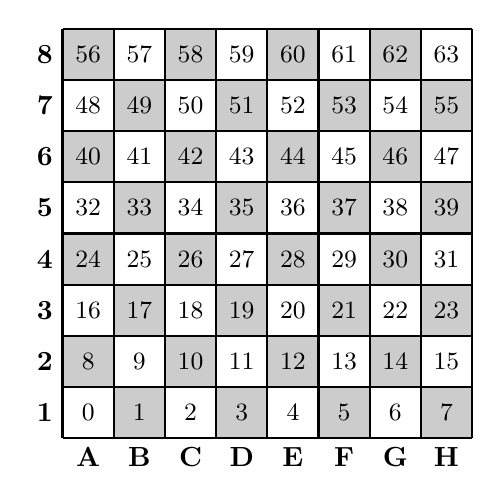
\begin{tikzpicture}[scale=0.65]
        % Draw the chessboard
        \foreach \x in {0,1,...,7} {
            \foreach \y in {0,1,...,7} {
                \pgfmathparse{mod(\x+\y,2) ? "black!20" : "white"}
                \edef\col{\pgfmathresult}
                \fill[\col] (\x,\y) rectangle (\x+1,\y+1);
                
                % Calculate the square index
                \pgfmathtruncatemacro{\num}{\x + 8*\y}
                % Add the number to the square
                \node at (\x+0.5,\y+0.5) {\small \num};
            }
        }

        % Add column labels (A-H)
        \foreach \x [count=\i from 0] in {A, B, C, D, E, F, G, H} {
            % \node[above] at (\i+0.5, 8) {\textbf{\x}}; % Top labels
            \node[below] at (\i+0.5, 0) {\textbf{\x}}; % Bottom labels
        }

        % Add row labels (1-8)
        \foreach \y [count=\i from 0] in {1, 2, 3, 4, 5, 6, 7, 8} {
            \node[left] at (0, \i+0.5) {\textbf{\y}}; % Left labels
            % \node[right] at (8, \i+0.5) {\textbf{\y}}; % Right labels
        }

        % Draw the grid
        \draw[thick] (0,0) grid (8,8);
    \end{tikzpicture}
    \caption{Little-Endian Rank-File Mapping with Coordinates.}
    \label{fig:lerf}
\end{figure}

\noindent \parbox{\textwidth}{There are bitboards for all pieces (\texttt{bitboard\_all}), for each piece color (\texttt{bitboard\_color[0]} and \texttt{bitboard\_color[1]}), and for each piece type (\texttt{bitboard\_piece[Piece]} like \texttt{bitboard\_piece[Piece::W\_QUEEN]})}.

\vspace{1em}

\noindent To identify ray directions on the board, we used the compass rose:

\begin{center}
    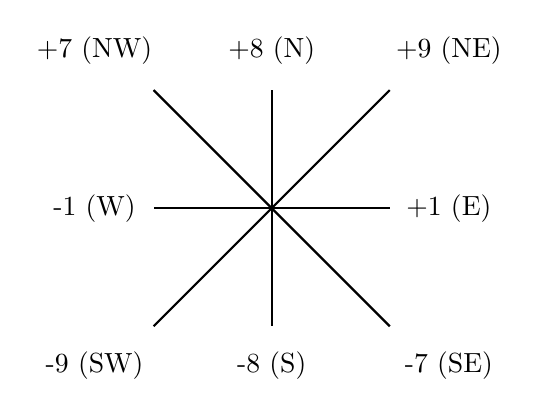
\begin{tikzpicture}
        \node at (0, 2) {+8 (N)};
        \node at (2.25, 2) {+9 (NE)};
        \node at (-2.25, 2) {+7 (NW)};
        \node at (2.25, 0) {+1 (E)};
        \node at (-2.25, 0) {-1 (W)};
        \node at (0, -2) {-8 (S)};
        \node at (2.25, -2) {-7 (SE)};
        \node at (-2.25, -2) {-9 (SW)};
        \draw[thick] (0, 0) -- (0, 1.5);
        \draw[thick] (0, 0) -- (1.5, 1.5);
        \draw[thick] (0, 0) -- (-1.5, 1.5);
        \draw[thick] (0, 0) -- (1.5, 0);
        \draw[thick] (0, 0) -- (-1.5, 0);
        \draw[thick] (0, 0) -- (0, -1.5);
        \draw[thick] (0, 0) -- (1.5, -1.5);
        \draw[thick] (0, 0) -- (-1.5, -1.5);
    \end{tikzpicture}
\end{center}

\noindent This means that, to get the numerical value that identifies the square to the north-east of a given square, you only need to add 9. For example, given the square $f6$ (45), the north-east square $g7$ has a value of 54 (45 + 9 = 54). It is really effective for sliding pieces to calculate their attacks.

\subsubsection{Transposition table}

The transposition table contains a list of entries. These entries are defined as a storage of information about a specific chess position, including its Zobrist key, evaluation score, best move, node type, and search depth.

\ldots

\subsubsection{History}

\ldots

\subsubsection{Move generator information}

\ldots

\subsection{Precomputed data}

Some tables are memory initialized instead of computed, explain it.

\ldots

\section{Additional tools and work}

\ldots

\subsection{Board visualizer using Python}

\ldots

\subsection{Profiling}

Continue in next Chapter~\ref{cap:profiling}.

\ldots

\subsection{Testing engine strength}

Testing and analysis in Chapter~\ref{cap:testing}.

\ldots
\chapter{Improvement Techniques}\label{cap:ImprovementTechniques}

This chapter documents the implementation of the following techniques used to improve the chess engine:

\begin{itemize}[itemsep=1pt]
    \item Transposition tables with zobrist hashing.
    \item Move generator with magic bitboards and PEXT instructions.
    \item Evaluation with king safety and piece mobility parameters.
    \item Multithread search.
    \item Search with Late move Reductions.
\end{itemize}
\section{Transposition Table}\label{sec:tt}

\noindent As discused in the previous chapter (see~\cref{sec:iterativeDeepening}), the basic implementation of the chess engine generates a large amount of redundant calculations due to the iterative deepening approach and also the concept of transpositions: situations in which the same board position is reached through different sequences of moves in the game tree.
\noindent~\cref{fig:transposition_example} illustrates a position that can arise through multiple move orders. Where the white king could go to the g3 square from multiple paths.

\begin{figure}
    \centering
    \begin{minipage}{0.6\textwidth}
        \centering
        \newchessgame
        \chessboard[
            showmover=false,
            setfen=8/2k5/3p4/p2P1p2/P2P1P2/8/8/2K5 w - - 0 1,
            pgfstyle=straightmove, color=blue,
            markmoves={c1-e3,e3-g3,c1-g1,g1-g3},
            arrow=to
        ]
    \end{minipage}
    \caption{Lasker-Reichhelm Position, transposition example}\label{fig:transposition_example}
\end{figure}

\vspace{1em}

\noindent Taking advantage of dynamic programming, we create a look-up table of chess positions and its evaluation. So if we encounter the same position again, the evaluation is already precalculated. However, we ask ourselves the following question: how much space does the look-up table take up if there are an astronomical amount of chess positions? What we can do is assign a hash to each position and make the table index the last bits of the hash. The larger the table, the less likely access collisions will be. We also want a hash that is fast to calculate and has collision-reducing properties.
~\cite{TranspositionTable}

\vspace{1em}

\noindent \parbox{\textwidth}{The complete implementation can be found in\\\texttt{include\textbackslash{}utilities\textbackslash{}transposition\_table.hpp}.}

\subsection{Zobrist Hashing}

Zobrist Hashing is a technique to transform a board position of arbitrary size into a number of a set length, with an equal distribution over all possible numbers invented by Albert Zobrist~\cite{ZobristHashing}.

\vspace{1em}

\noindent To generate a 64-bit hash for a position, the following steps are followed:

\begin{enumerate}
  \item Pseudorandom 64-bit numbers are generated for each possible feature of a position:
  \begin{enumerate}
    \item One number for each piece type on each square — 12 pieces x 64 squares = 768 numbers.
    \item One number to indicate the side to move is black.
    \item Four numbers to represent castling rights (kingside and queenside for both white and black).
    \item Eight numbers to represent the file of an available \textit{en passant} square.
  \end{enumerate}
  \item The final hash is computed by XOR-ing together all the random numbers corresponding to the features present in the current position.
\end{enumerate}

\noindent These random values ensure that even slightly different positions produce very different hash values. This greatly reduces the chance of collisions.

\vspace{1em}

\noindent The XOR operation is used not only because it is computationally inexpensive, but also because it is reversible. This means that when a move is made or undone, we can update the hash incrementally by applying XOR only to the affected squares, without needing to recompute the entire hash.

\vspace{1em}

\noindent The position shown in~\cref{fig:zobristExamplePosition} illustrates an example of how the Zobrist hash is computed.  
The hash value is calculated by XORing the random values associated with each element of the position.  
Since the side to move is White, we do not XOR the value associated with Black to move.  
The resulting hash is computed as follows:

\[
111 \oplus 69 \oplus 909 \oplus 10 \oplus 67 \oplus 12 \oplus 555 \oplus 3 = 458
\]

\noindent Where $\oplus$ denotes $XOR$.

\begin{figure}
    \centering
    \begin{minipage}[t]{0.4\textwidth}
        \centering
        \newchessgame
        \chessboard[
            showmover=true,
            setfen=7r/8/k7/1pP5/8/4Q3/1P6/1K6 w - b6 0 1,
            markstyle=circle,
            color=blue, markfields={b6},
            pgfstyle=straightmove, color=red,
            markmoves={b7-b5},
            arrow=to
        ]
        \caption*{Side to move is white. The last move was a pawn advancing from b7 to b5, making \text{en passant} available on the b6 square.}
    \end{minipage}
    \hspace{1cm}
    \begin{minipage}[t]{0.4\textwidth}
        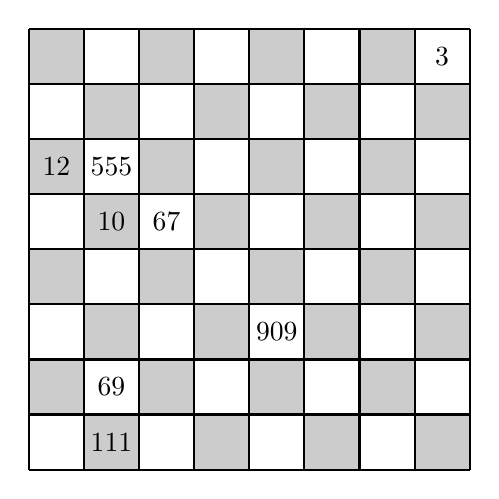
\begin{tikzpicture}[scale=0.7]

            \foreach \x in {0,1,...,7} {
                \foreach \y in {0,1,...,7} {
                    \pgfmathparse{mod(\x+\y,2) ? "black!20" : "white"}
                    \edef\col{\pgfmathresult}
                    \fill[\col] (\x,\y) rectangle (\x+1,\y+1);
                }
            }

            \node at (1.5,0.5) {111}; \node at (1.5,1.5) {69}; \node at (4.5,2.5) {909}; \node at (1.5,4.5) {10};
            \node at (2.5,4.5) {67}; \node at (0.5,5.5) {12}; \node at (1.5,5.5) {555}; \node at (7.5,7.5) {3};

            \draw[thick] (0,0) grid (8,8);
        \end{tikzpicture}
        \vspace{1.5em}
        \caption*{Random values corresponding to each piece and the en passant square. The value for Black to move is 62319.}
    \end{minipage}
    \caption{Zobrist hash calculation example.}\label{fig:zobristExamplePosition}
\end{figure}

\subsection{Table Entry}

Each entry in the transposition table stores the following information:

\begin{enumerate}
  \item \textit{Zobrist Hash}: The full 64-bit hash of the position. This is used to verify that the entry corresponds to the current position and to detect possible index collisions in the table.
  \item \textit{Evaluation}: The numerical evaluation of the position, as computed by the evaluation function.
  \item \textit{Depth}: The depth at which the evaluation was calculated. A deeper search could potentially yield a more accurate evaluation, so this value helps determine whether a new evaluation should overwrite the existing one.
  \item \textit{Node Type}: Indicates the type of node stored:
  \begin{enumerate}
    \item \textit{EXACT} the evaluation is precise for this position.
    \item \textit{UPPERBOUND} the evaluation is an upper bound, typically resulting from an alpha cutoff.
    \item \textit{LOWERBOUND} the evaluation is a lower bound, typically resulting from a beta cutoff.
    \item \textit{FAILED} entry is empty or with invalid information.
  \end{enumerate}
\end{enumerate}

\subsection{Collisions}

As discussed earlier, index collisions in the transposition table are handled by verifying the full Zobrist hash stored in the entry. However, it is still theoretically possible for a full hash collision to occur, that is two different positions producing the same hash.

\vspace{1em}

\noindent This scenario is extremely rare. With 64-bit hashes, there are $2^{64}$ possible unique values, which is more than sufficient for practical purposes. In the unlikely event of a true hash collision, it could result in an incorrect evaluation being reused for a different position.

\section{Move generator with Magic Bitboards and PEXT instructions}

To identify potential performance bottlenecks, we performed profiling on the engine, as shown in~\cref{fig:profiling}.

\vspace{1em}

\begin{figure}
    \centering
    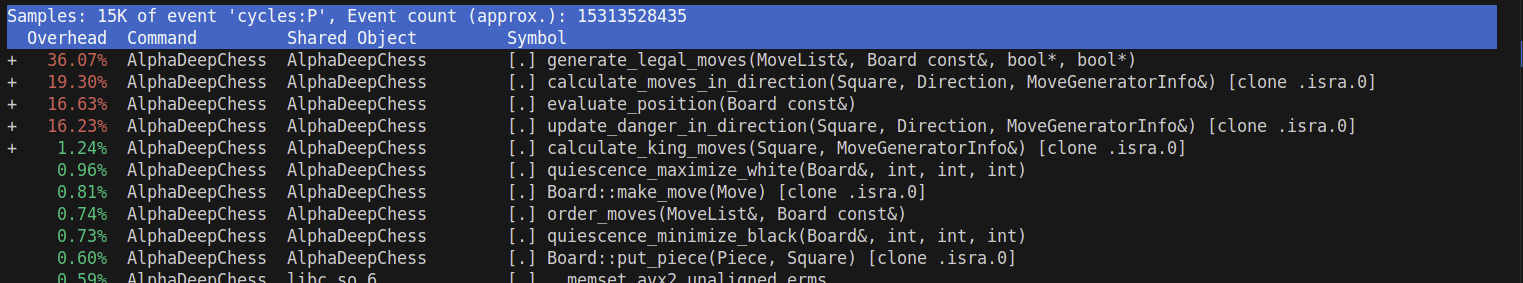
\includegraphics[width=1.0\textwidth]{Imagenes/basic_move_generator_profiling.png}
    \caption{Profiling results.}\label{fig:profiling}
\end{figure}

\noindent The profiling results indicate that the majority of the total execution time is spent in the legal move generation function. Therefore, optimizing this component is expected to yield significant performance improvements.

\subsection{Magic bitboards}

We can create a look up table of all the rook and bishop moves for each square on the board and for each combination of pieces that blocks the path of the slider piece (blockers  bitboard). Basically we need a hash table to store rook and bishop moves indexed by square and bitboard of blockers. The problem is that this table could be very big~\cite{MagicBitboards}.

\vspace{1em}

\noindent Magic bitboards technique used to reduce the size of the look up table. We cut off unnecesary information in the blockers bitboard, excluding the board borders and the squares outside its attack pattern.

\vspace{1em}

\noindent A \textbf{magic number} is a multiplier to the bitboard of blockers with the following properties:

\begin{itemize}[itemsep=1pt]
  \item Preserves relevant blocker information: 
  The nearest blockers along a piece's movement direction are preserved. 
  \textit{Example:} Consider a rook with two pawns in its path:
  \begin{center}
    Rook $\rightarrow \rightarrow \rightarrow$ [Pawn1][Pawn2]
  \end{center}
  In this case, only `Pawn1` blocks the rook's movement, while `Pawn2` is irrelevant.
  \item Compresses the blocker bitboard, pushing the important bits near the most significant bit.
  \item The final multiplication must produce a unique index for each possible blocker configuration. The way to ensure the uniqueness is by brute force testing.
\end{itemize}

\noindent As illustrated in~\ref{fig:magics_position}, we aim to compute the legal moves of the white rook in the given position. In practice, the only pieces that truly block the rook's path are those marked with a red circle.

\vspace{1em}

\begin{figure}
    \centering
    \begin{minipage}{0.6\textwidth}
        \centering
        \newchessgame
        \chessboard[
            showmover=false,
            setfen=n1bk3r/3p4/1p1p2p1/8/3R1p2/8/3p4/7n w - - 0 1,
            markstyle=circle,
            color=red, markfields={d6,f4,d2},
            color=green, markfields={c4,b4,a4,e4,d5,d3}
        ]
    \end{minipage}
    \caption{Initial chess position with white rook and blockers}\label{fig:magics_position}
\end{figure}

\subsection*{Magic number generation}

\noindent
Magic numbers are generated through a trial and error process. For each square on the board,random numbers are tested until one produces a unique index for every possible blocker configuration~\cite{MagicBitboards}. Over the years, the chess programming community has discovered better magic numbers. In this project, we use magics sourced from the Chess Programming YouTube channel~\cite{MagicsSource}.


\subsection*{Index calculation}

\noindent First, we mask out all pieces outside the rook's attack pattern or on the board borders, as shown in~\ref{fig:magic_preprocessing}.

\vspace{1em}

\begin{figure}
    \centering
    \begin{minipage}[c]{0.4\textwidth}
        \centering
        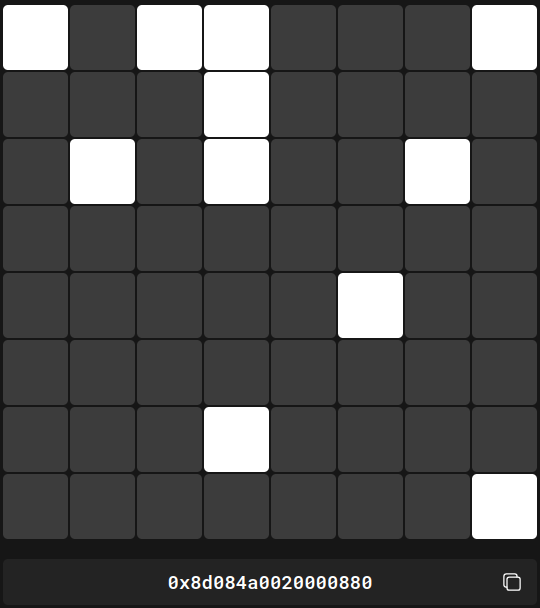
\includegraphics[width=\textwidth]{Imagenes/magics_blockers.png}
        \caption{Original blockers bitboard}
    \end{minipage}
    \hfill
    \begin{minipage}[c]{0.1\textwidth}
        \centering
        \small$\to$
    \end{minipage}
    \hfill
    \begin{minipage}[c]{0.4\textwidth}
        \centering
        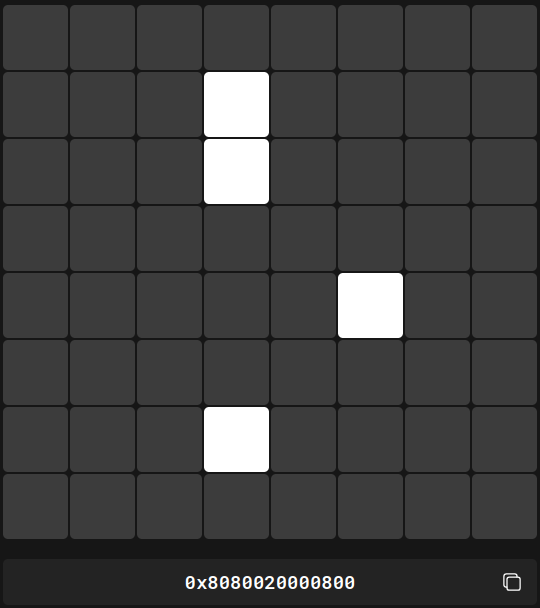
\includegraphics[width=\textwidth]{Imagenes/magics_processed_blockers.png}
        \caption{Masked blockers bitboard}
    \end{minipage}
    \caption{Pre-processing of the blockers bitboard}\label{fig:magic_preprocessing}
\end{figure}

\noindent As illustrated in~\ref{fig:magic_multiplication}, the masked blockers bitboard is then multiplied by the magic number. The result retains only the three relevant pawns that obstruct the rook's movement, pushing them toward the most significant bits.

\vspace{1em}

\begin{figure}
    \centering
    \begin{minipage}[c]{0.4\textwidth}
        \centering
        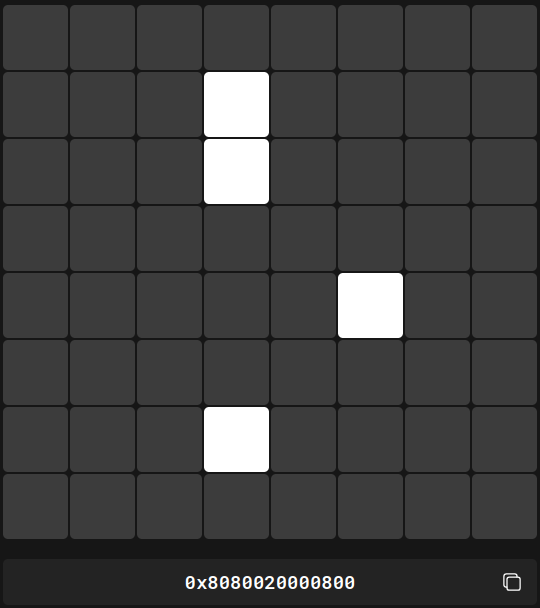
\includegraphics[width=\textwidth]{Imagenes/magics_processed_blockers.png}
        \caption{Masked blockers bitboard}
    \end{minipage}
    \hfill
    \begin{minipage}[c]{0.1\textwidth}
        \centering
        \Huge$\times$ \\[0.5em]
        \small Magic number \\[0.5em]
        \Huge$=$
    \end{minipage}
    \hfill
    \begin{minipage}[c]{0.4\textwidth}
        \centering
        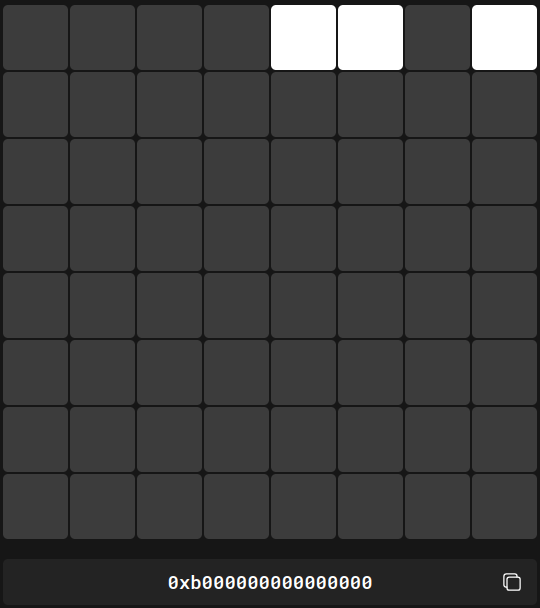
\includegraphics[width=\textwidth]{Imagenes/magics_multiplied_blockers.png}
        \caption{Multiplied blockers bitboard}
    \end{minipage}
    \caption{Multiplication by magic number to produce an index}\label{fig:magic_multiplication}
\end{figure}

\noindent Next, we compress the index toward the least significant bits by shifting right by \(\,64-\)\texttt{relevant\_squares}. The number of relevant squares varies per board square; ~\ref{fig:rook_relevant_squares} shows this for the rook:

\vspace{1em}

\begin{figure}
    \centering
    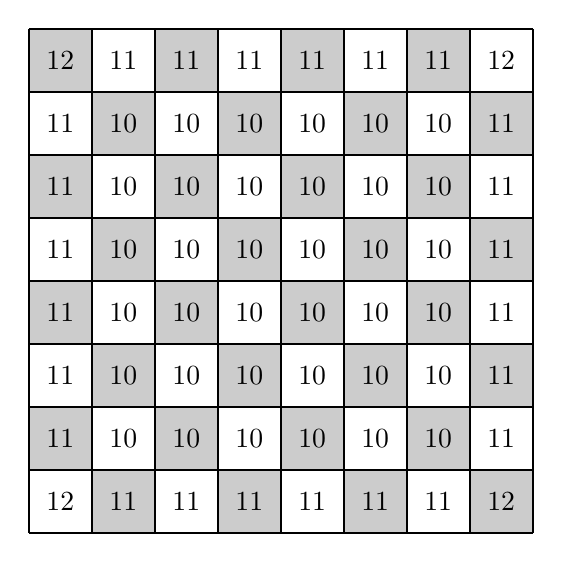
\begin{tikzpicture}[scale=0.8]
        % Draw the chessboard
        \foreach \x in {0,1,...,7} {
            \foreach \y in {0,1,...,7} {
                \pgfmathparse{mod(\x+\y,2) ? "black!20" : "white"}
                \edef\col{\pgfmathresult}
                \fill[\col] (\x,\y) rectangle (\x+1,\y+1);
            }
        }

        % Add the values to the squares
        \node at (0.5,7.5) {12}; \node at (1.5,7.5) {11}; \node at (2.5,7.5) {11}; \node at (3.5,7.5) {11};
        \node at (4.5,7.5) {11}; \node at (5.5,7.5) {11}; \node at (6.5,7.5) {11}; \node at (7.5,7.5) {12};

        \node at (0.5,6.5) {11}; \node at (1.5,6.5) {10}; \node at (2.5,6.5) {10}; \node at (3.5,6.5) {10};
        \node at (4.5,6.5) {10}; \node at (5.5,6.5) {10}; \node at (6.5,6.5) {10}; \node at (7.5,6.5) {11};

        \node at (0.5,5.5) {11}; \node at (1.5,5.5) {10}; \node at (2.5,5.5) {10}; \node at (3.5,5.5) {10};
        \node at (4.5,5.5) {10}; \node at (5.5,5.5) {10}; \node at (6.5,5.5) {10}; \node at (7.5,5.5) {11};

        \node at (0.5,4.5) {11}; \node at (1.5,4.5) {10}; \node at (2.5,4.5) {10}; \node at (3.5,4.5) {10};
        \node at (4.5,4.5) {10}; \node at (5.5,4.5) {10}; \node at (6.5,4.5) {10}; \node at (7.5,4.5) {11};

        \node at (0.5,3.5) {11}; \node at (1.5,3.5) {10}; \node at (2.5,3.5) {10}; \node at (3.5,3.5) {10};
        \node at (4.5,3.5) {10}; \node at (5.5,3.5) {10}; \node at (6.5,3.5) {10}; \node at (7.5,3.5) {11};

        \node at (0.5,2.5) {11}; \node at (1.5,2.5) {10}; \node at (2.5,2.5) {10}; \node at (3.5,2.5) {10};
        \node at (4.5,2.5) {10}; \node at (5.5,2.5) {10}; \node at (6.5,2.5) {10}; \node at (7.5,2.5) {11};

        \node at (0.5,1.5) {11}; \node at (1.5,1.5) {10}; \node at (2.5,1.5) {10}; \node at (3.5,1.5) {10};
        \node at (4.5,1.5) {10}; \node at (5.5,1.5) {10}; \node at (6.5,1.5) {10}; \node at (7.5,1.5) {11};

        \node at (0.5,0.5) {12}; \node at (1.5,0.5) {11}; \node at (2.5,0.5) {11}; \node at (3.5,0.5) {11};
        \node at (4.5,0.5) {11}; \node at (5.5,0.5) {11}; \node at (6.5,0.5) {11}; \node at (7.5,0.5) {12};

        % Draw the grid
        \draw[thick] (0,0) grid (8,8);
    \end{tikzpicture}
    \caption{Relevant squares for rook piece.}\label{fig:rook_relevant_squares}
\end{figure}

\noindent The final index is thus computed as:

\begin{align*}
    \text{index} 
    &= (\text{bitboard\_of\_blockers} \times \text{magic\_number})
       \;\gg\;(64 - \text{relevant\_squares})\,.
\end{align*}

\subsection{PEXT instruction}

\noindent The \texttt{PEXT} (Parallel Bits Extract) instruction—available on modern x86\_64 CPUs—extracts bits from a source operand according to a mask and packs them into the lower bits of the destination operand~\cite{PextInstruction}. It is ideally suited for computing our table index.

\vspace{1em}

\noindent\cref{fig:pext_instruction_example} illustrates how \texttt{PEXT} works: it selects specific bits from register \texttt{r2}, as specified by the mask in \texttt{r3}, and packs the result into the lower bits of the destination register \texttt{r1}.

\vspace{1em}

\begin{figure}
    \centering
    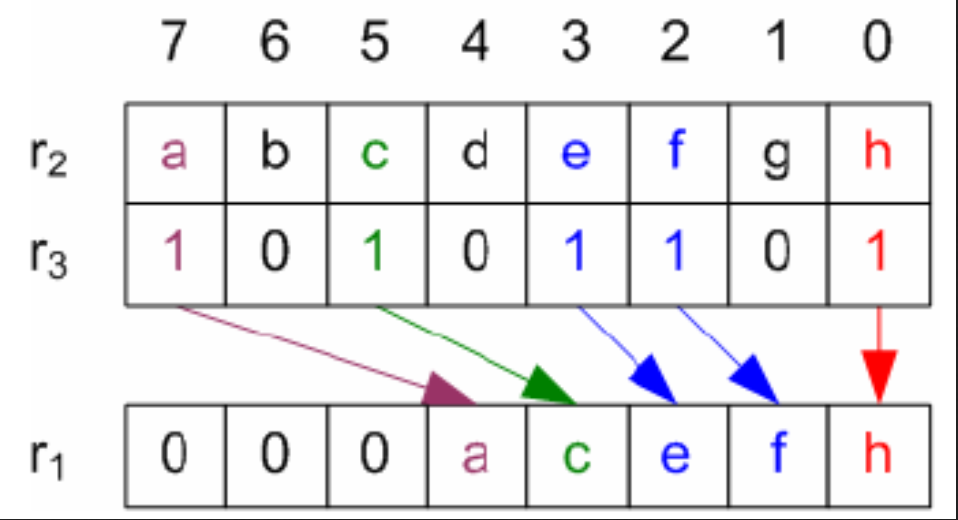
\includegraphics[width=0.5\textwidth]{Imagenes/pext.png}
    \caption{Example of the \texttt{PEXT} instruction.}\label{fig:pext_instruction_example}
\end{figure}

\noindent For our previous example (see~\cref{fig:magics_position}), we only need the full bitboard of blockers and the rook’s attack pattern (excluding the borders to reduce space), as illustrated in~\cref{fig:pext_bitboards}.

\vspace{1em}

\begin{figure}
    \centering
    \begin{minipage}[c]{0.3\textwidth}
        \centering
        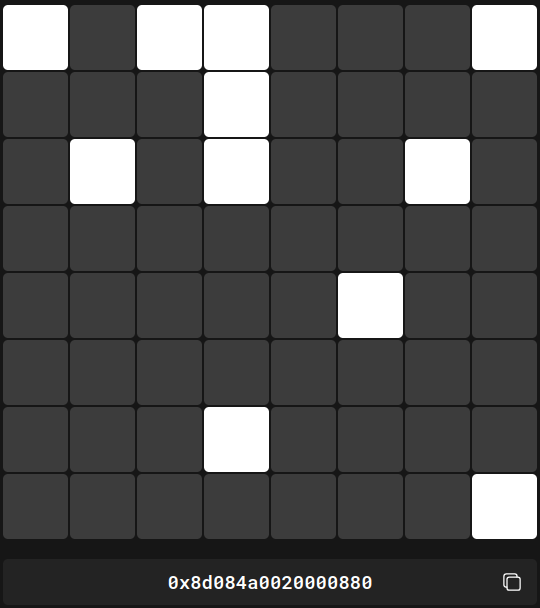
\includegraphics[width=\textwidth]{Imagenes/magics_blockers.png}
        \caption{Blockers bitboard}
    \end{minipage}
    \hfill
    \begin{minipage}[c]{0.3\textwidth}
        \centering
        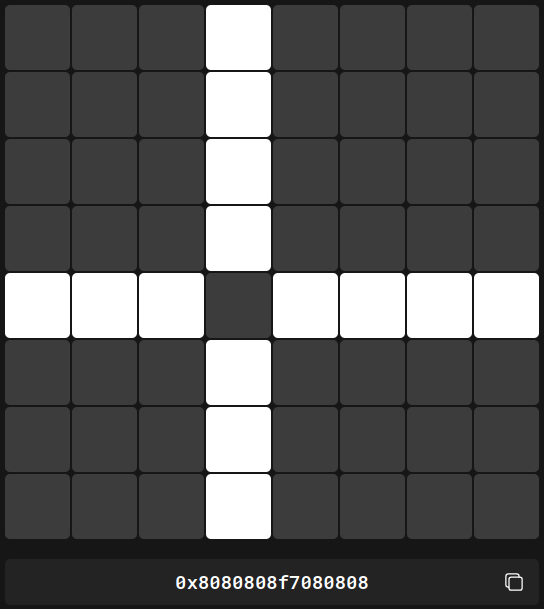
\includegraphics[width=\textwidth]{Imagenes/magics_rook_attacks.png}
        \caption{Rook attack mask}
    \end{minipage}
    \hfill
    \begin{minipage}[c]{0.05\textwidth}
        \centering
        \Huge\texttt{->}
    \end{minipage}
    \hfill
    \begin{minipage}[c]{0.3\textwidth}
        \centering
        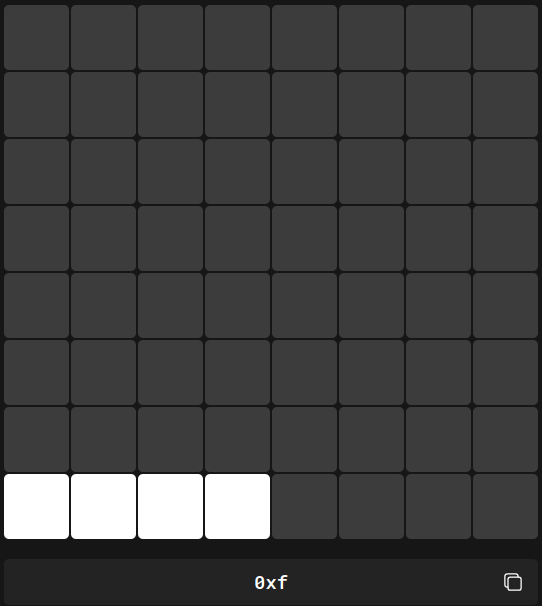
\includegraphics[width=\textwidth]{Imagenes/pext_final_index.png}
        \caption{Final extracted index}
    \end{minipage}
    \caption{index extraction with Pext example}\label{fig:pext_bitboards}
\end{figure}

\noindent The final index used to access the lookup table is calculated using the \texttt{pext} instruction as follows:
\begin{align*}
    \text{index}
    &= \text{\_pext\_u64}(\text{blockers},\,\texttt{attack\_pattern})\,.
\end{align*}

\subsection*{Conditional implementation}

\noindent To maintain compatibility and performance across different hardware platforms, we provide two implementations for computing the indices:

\begin{itemize}[itemsep=1pt]
  \item If \texttt{PEXT} support is detected at compile time, the engine uses it to compute the index directly.
  \item Otherwise, the engine falls back to the magic bitboards approach using multiplication and bit shifts.
\end{itemize}

\newpage

\section{Evaluation with King Safety and piece mobility}

While material count is the fundamental part for evaluating a chess position, human players also consider strategic and positional factors such as pawn structure, piece activity and king safety. We extend the evaluation function by incorporating additional parameters. These enhancements aim to produce a more accurate assessment of the position.

\subsection*{King shield bonus}

The king is typically safer when protected by friendly pawns in front of it. We assign a bonus in the evaluation score for each allied pawn positioned directly in front of the king. In the following image the white side has one pawn in front of the king, adding 100 bonus points, while black has 3 pawns adding 300 bonus shield points.

\begin{center}
    \newchessgame
    \chessboard[
        showmover=false,
        setfen=r1b2rk1/1ppp1ppp/2n5/p1b1p2n/2B1P2q/2NP1N2/PPP2P2/R1BQ1RK1 b - - 7 15,
        markstyle=border,
        color=green, markfields={f2},
        color=blue, markfields={f7,g7,h7}
    ]
\end{center}

\subsection*{King Safety Penalty}

To evaluate the safety of the king, we analyze the $3 \times 3$ area surrounding the king, counting how many enemy pieces attack any of those squares. Each type of attacking piece contributes a different \textit{threat weight}:

\begin{itemize}
    \item Queen: 4 points.
    \item Rook: 3 points.
    \item Bishop/Knight: 2 points.
    \item Pawn: 1 point.
\end{itemize}

\par We sum these threat values to compute a \textit{total danger score}. This score is then used as an index into the \textit{precomputed safety table}~\cref{tab:safetyTable}, which returns the corresponding penalty to apply to the evaluation score. This method allows us to smoothly scale the penalty based on the level of threat around the king. The maximum penalty applied is 500 points.

\begin{table}
\centering
\caption{Sample entries from the king safety penalty table.}
\begin{tabular}{|c|c|c|c|c|c|c|c|c|c|c|}
\hline
\textit{Threat Score}     & 0 & 1 & 2 & 3 & 5 & 10 & ... & 20 & ... & 61 \\
\hline
\textit{Penalty} & 0 & 0 & 1 & 2 & 5 & 18 & ... & 68 & ... & 500 \\
\hline
\end{tabular}
\label{tab:safetyTable}
\end{table}

\par In the following image, the black king is under threat from multiple pieces: the queen attacks two squares (8 points), the rook attacks three squares (9 points), a knight attacks one square (2 points), and a pawn attacks one square (1 point). This results in a total threat score of 20, which corresponds to a penalty of 68 points according to the safety table.


\begin{center}
    \newchessgame
    \chessboard[
        showmover=false,
        setfen=7k/5pnp/1p6/p2P4/2Np4/8/8/K1Q4R w - - 0 1,
        markstyle=border,
        color=green, markfields={g8,f8,e8,e7,f7,g7,f6,g6,f5},
        color=red, markfields={h5,h6,h7,e6,e5,g5}
    ]
\end{center}

\subsection*{Piece mobility}

Greater piece mobility is generally indicative of a stronger position. Each piece receives a bonus for every available move to a square that is not attacked by enemy pawns. 

\vspace{1em}

To implement this feature, we first compute a bitboard representing all legal moves available to a given piece. We then apply a mask that removes any squares attacked by enemy pawns. The resulting bitboard contains only safe mobility squares. For example in the following image the queen has twelve legal moves to squares not attacked by enemy pawns, and therefore receives a mobility bonus of 12 points. The safe squares are highlighted in green.

\begin{center}
    \newchessgame
    \chessboard[
        showmover=false,
        setfen=rn2kbnr/pppbpppp/8/3q4/7P/8/PPPP1PP1/RNBQKBNR b KQkq - 0 1,
        markstyle=border,
        color=red, markfields={g5,f3,d3,b3},
        color=green, markfields={d4,d6,e5,f5,h5,c5,b5,a5,c4,e6,c6,e4}
    ]
\end{center}

\section{Multithreaded Search}

This version of search follows Young Brothers Wait Concept, which is a parallel search algorithm designed to optimize the distribution of work among multiple threads.

\vspace{1em}

\noindent This is particularly effective in alpha-beta pruning, where the search tree is explored selectively. It is divided into two phases: the principal variation move and the wait concept.

\vspace{1em}

\noindent The principal variation is searched sequentially by the main thread, ensuring that the most promising move is evaluated first. If this move turns out to be the best and pruning is applied, the search can directly return the final node evaluation. Otherwise, once the first move has been evaluated, the remaining moves are distributed among multiple threads for parallel evaluation. The wait concept refers to these threads that remain idle until the main thread finishes searching the principal variation.

\vspace{1em}

\noindent In~\cref{fig:pvsplitting}, the gray circle and square nodes are considered part of the principal variation, while the remaining white nodes are processed in parallel by multiple threads.

\begin{figure}
   \centering
   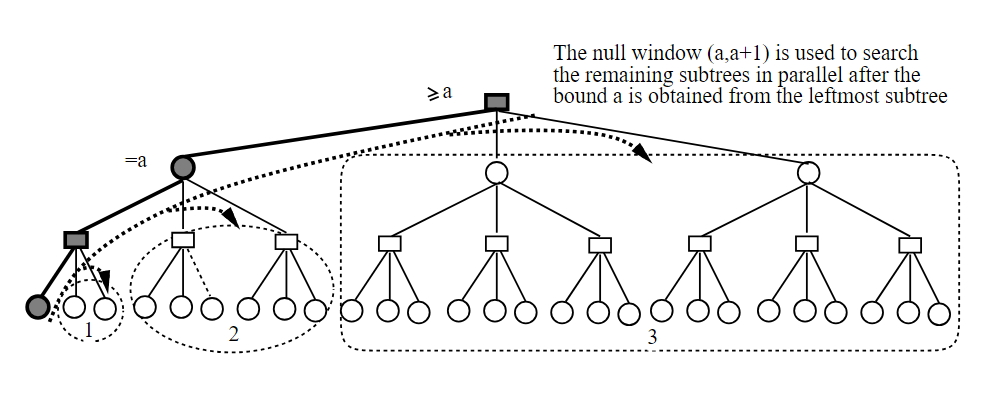
\includegraphics[width=0.8\textwidth]{Imagenes/Bitmap/pvsplitting.png}
   \caption{Principal variation splitting~\cite{PVSplitting}.}\label{fig:pvsplitting}
\end{figure}

\newpage
\section{Late Move Reductions}

\noindent We experiment with the use of late move reductions, a search optimization technique that selectively reduces the search depth for moves that appear late in the move ordering and are therefore considered less promising~\cite{LateMoveReductions}. The technique is based on the assumption that a strong move ordering heuristic will place the best move in the position earlier in the list. As a result, moves evaluated later can be searched at a reduced depth to save computation time.

\vspace{1em}

\par
In our implementation, a reduction of one ply is applied to non-capturing moves when the side to move is not in check, the remaining search depth is at least three plies, and the move index is beyond a threshold of the 10th move. The reduction condition is formally defined in Equation~\ref{eq:lmr}:

\vspace{1em}

\begin{equation}
\text{reduction} = 
\begin{cases}
1, & \text{if } \text{isNotCheck} \wedge \text{depth} \geq 3 \wedge moveIndex \geq 10 \\
0, & \text{otherwise}
\end{cases}
\label{eq:lmr}
\end{equation}

\vspace{1em}

\par
If the reduced-depth search returns a score within the alpha-beta window ($\alpha < \text{eval} < \beta$), indicating that the move may be stronger than initially assumed, a full-depth re-search is triggered to ensure it is not mistakenly pruned.



\chapter{Analysis and evaluation}\label{cap:analysis}

This chapter presents an analysis of the performance of the chess engine through profiling, identifying its most computationally intensive components. We then describe the testing framework used to evaluate the effectiveness of the optimization techniques introduced in~\cref{cap:ImprovementTechniques}. These evaluations are based on 100-game matches between different versions of the engine and a baseline implementation. Finally, we compare the performance of \textit{AlphaDeepChess} against \textit{Stockfish} and examine its position within the Elo rating distribution on \textit{Lichess.org}.

\section{Profiling}
In order to analyze the performance of our chess engine and identify potential bottlenecks where the code consume the most execution time, we used the \texttt{perf} tool available on Linux systems. \texttt{perf} provides robust profiling capabilities by recording CPU events, sampling function execution, and collecting stack traces~\cite{PerfLinux}. 

\vspace{1em}

\noindent We run the engine under \texttt{perf} using the following commands:

\begin{lstlisting}[language=bash, caption={Profiling \textit{AlphaDeepChess} with perf}, frame=single, breaklines=true, captionpos=b]
# Record performance data with function stack traces
sudo perf record -g ./build/release/AlphaDeepChess

# Display interactive report
sudo perf report -g --no-children
\end{lstlisting}

\noindent After recording, \texttt{perf report} opens an interactive terminal interface where functions are sorted by CPU overhead, allowing us to easily identify performance-critical regions.

\vspace{1em}

\noindent First, we profile the basic architecture of the engine implemented in~\cref{cap:descripcionTrabajo}, and then evaluate it again after applying the optimizations described in~\cref{cap:ImprovementTechniques}.

\subsection*{Profiling of basic engine architecture}

\noindent As shown in~\cref{tab:profilingBasic}, the profiling results indicate that the majority of the total execution time is spent in the legal move generation function. Specifically, the functions \texttt{generate\_legal\_moves}, \texttt{calculate\_moves\_in\_dir}, and \texttt{update\_danger\_in\_dir} together account for over 72\% of the total overhead. Therefore, the optimizations on this component are expected to yield significant performance improvements.

\begin{table}[H]
    \centering
    \begin{tabular}{|l|r|}
    \hline
    \textit{Symbol} & \textit{Overhead} \\
    \hline
    \texttt{generate\_legal\_moves}       &  36.07\% \\
    \texttt{calculate\_moves\_in\_dir}    &  19.30\% \\
    \texttt{evaluate\_position}          &  16.63\% \\
    \texttt{update\_danger\_in\_dir}      &   16.23\% \\
    \texttt{calculate\_king\_moves}       &   1.24\% \\
    \texttt{quiescence\_search}          &   0.96\% \\
    \texttt{...}                          &   ...     \\
    \hline
    \end{tabular}
    \caption{Profiling results of the basic engine implementation.}
    \label{tab:profilingBasic}
\end{table}

\vspace{1em}

\subsection*{Profiling with improvement techniques}

\noindent As shown in~\cref{tab:profilingImprovements}, the updated profiling results demonstrate a successful reduction in the computational cost of move generation. The execution time is now more evenly distributed across various modules, with position evaluation emerging as the new primary performance bottleneck. This shift confirms the effectiveness of the implemented optimization techniques.

\begin{table}[H]
    \centering
    \begin{tabular}{|l|r|}
    \hline
    \textit{Symbol} & \textit{Overhead} \\
    \hline
    \texttt{evaluate\_position}       &  31.90\% \\
    \texttt{update\_attacks\_bb}    &  22.62\% \\
    \texttt{generate\_legal\_moves}          &  22.71\% \\
    \texttt{order\_moves}      &   3.95\% \\
    \texttt{make\_move}       &   3.83\% \\
    \texttt{alpha\_beta\_search}          &   1.66\% \\
    \texttt{...}                          &   ...     \\
    \hline
    \end{tabular}
    \caption{Profiling results after applying optimization techniques.}
    \label{tab:profilingImprovements}
\end{table}

\section{Testing framework}

\noindent In this section, we describe the tools used to test and debug the engine, as well as the methodology for evaluating each of the improvement techniques implemented throughout the development of the chess engine.

\subsection*{Graphical user interface}

\noindent Although we implemented a \texttt{diagram} command to display the current position in the standard output, making moves and observing evaluations can be a time-consuming process during debugging and testing. To streamline this workflow, we developed a graphical user interface (GUI) using Python. For rapid development and ease of use, we chose \textit{CustomTkinter}, one of the most widely adopted Python UI libraries.

\vspace{1em}

\parbox{\textwidth}{\noindent The GUI provides a user-friendly interface that communicates with the engine using the UCI protocol under the hood, greatly enhancing the debugging and testing experience. This tool can be used after compiling the engine by running \texttt{AlphaDeepChessGUI.py} with Python.}


\begin{figure}[H]
    \centering
    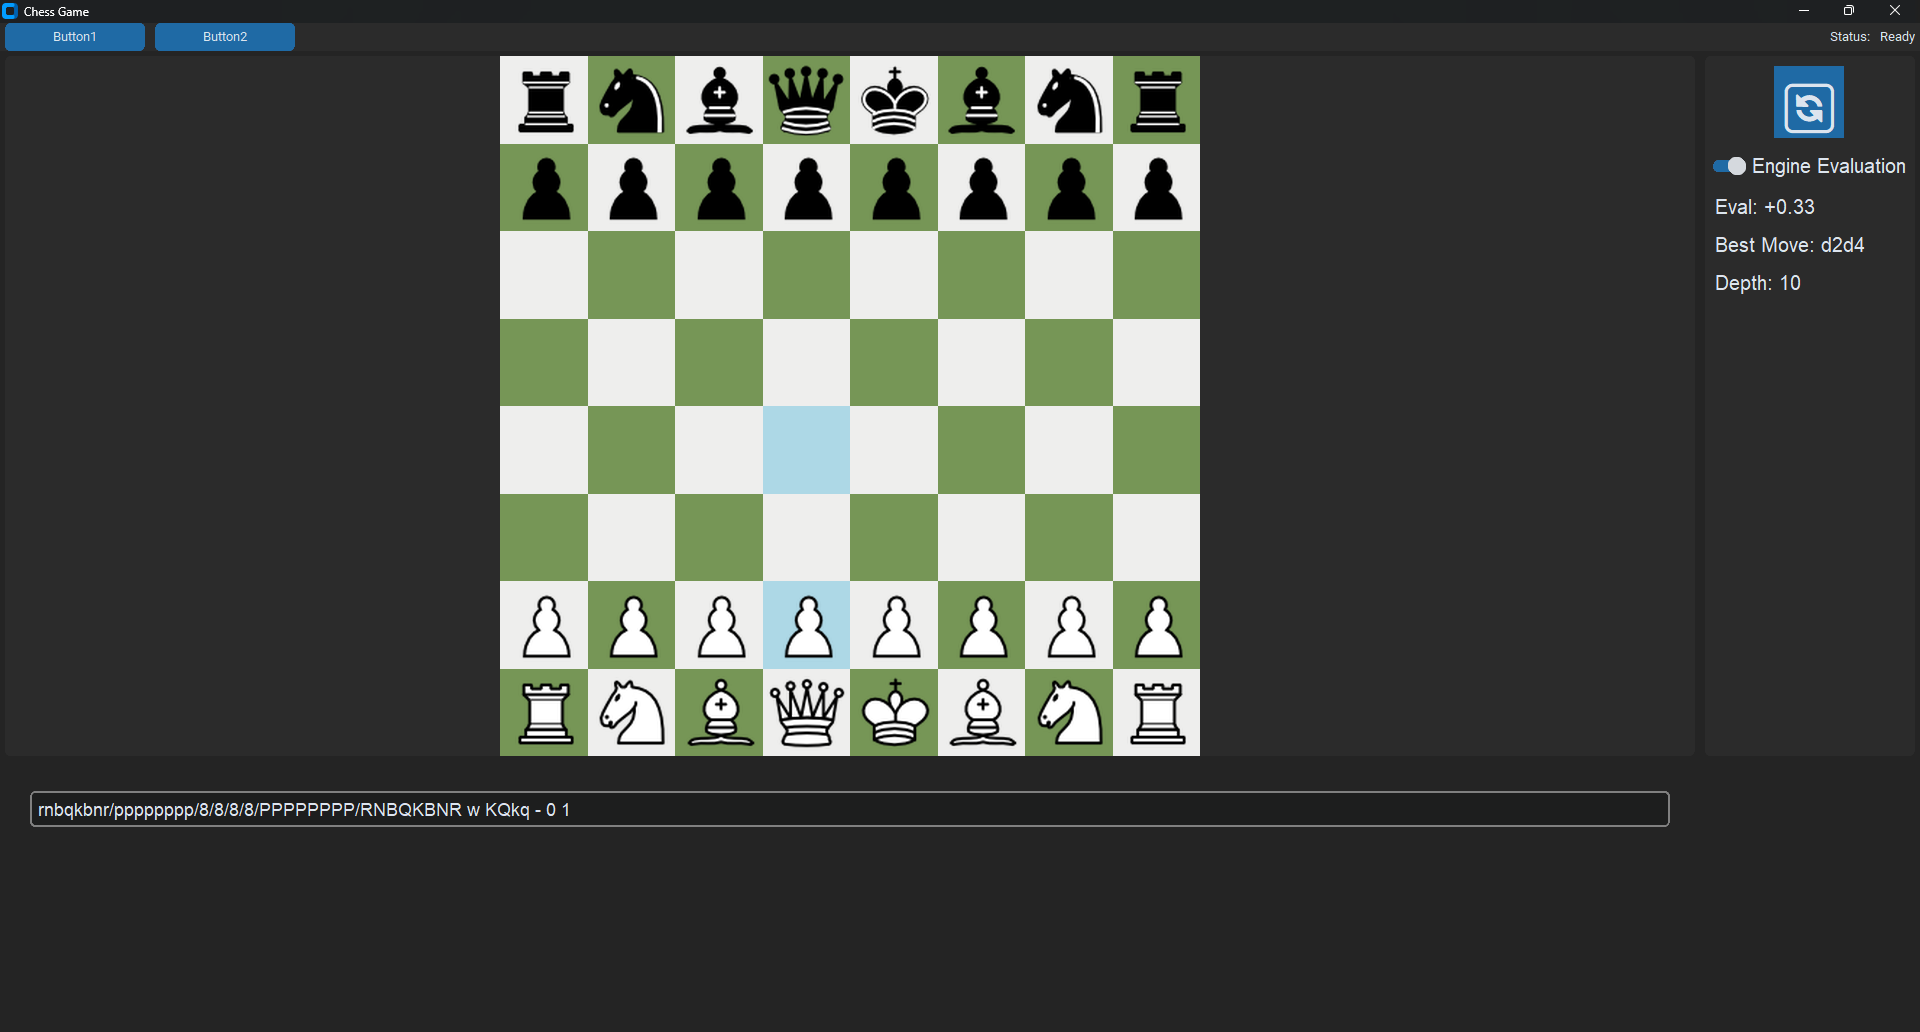
\includegraphics[width=1.0\textwidth]{Imagenes/gui.png}
    \caption{\textit{AlphaDeepChess}'s GUI}\label{fig:gui}
\end{figure}

\noindent In~\cref{fig:gui}, the engine evaluation is enabled and displays the current evaluation value, the best move found, and the calculated search depth. In this way, we also ensure a more user-friendly experience.


\subsection*{\textit{Cutechess}}

\noindent To evaluate the different techniques implemented, we also required a tool capable of running automated tournaments between chess engines. For this task, we used \textit{Cutechess}, whose usage is described in detail in~\cref{sec:cutechess}.

\vspace{1em}

\noindent Depending on the number of games, search time, and time control, these tournaments between engines can take a long time to process. For this reason, we decided to use GitHub Actions and workflows to separate our development environment from the execution of performance and strength tests.

\vspace{1em}

\subsection*{Github actions and workflows}

GitHub Actions is a CI/CD tool integrated into GitHub that allows developers to automate tasks such as building, testing, and deploying code. Workflows are defined in YAML files and specify the tasks to be executed, the jobs or events that trigger them, and the environment in which they run.

\vspace{1em}

\parbox{\textwidth}{\noindent In this project, since it is public in a GitHub repository, we used GitHub Actions to automate the testing and evaluation of the chess engine with \textit{Stockfish} and \textit{Cutechess}. A workflow was configured (located at \texttt{.github\textbackslash{}workflows\textbackslash{}manual-workflow.yml}) to compile the engine and run automated games using \textit{Cutechess} between different versions of the engine or against \textit{Stockfish}.}

\section{Evaluation of improvements}

\noindent In this section we provide the results of a 100-game match between improved engine versions and a baseline version. The purpose of these matches is to measure the improvement in playing strength introduced by each new implementation. All matches are conducted using the tournament manager \textit{Cutechess} with the following configuration:

\begin{enumerate}
    \item 50 unique random starting positions, each played twice with alternating colors.
    \item 4 seconds of thinking time per move.
    \item A 150-move limit per game, after which the game is declared a draw.
\end{enumerate}

\vspace{1em}

\parbox{\textwidth}{The matches were executed on virtual machines provided by \textit{GitHub Actions}, using the ubuntu-latest runner. At the time of testing, this environment provided 4 CPUs, 16 GB of RAM, a 14 GB SSD, and a 64-bit architecture.}

\vspace{1em}

\noindent The baseline engine configuration is shown in~\cref{tab:baselineBot}. It includes only the core techniques described in~\cref{cap:descripcionTrabajo}.

\begin{table}[H]
    \centering
    \begin{tabular}{|p{4cm}|p{4cm}|}
    \hline
    \textit{Component}         & \textit{Baseline Bot}     \\ \hline
    Search                     & Basic Alpha-Beta           \\ \hline
    Evaluation Function        & Materialistic        \\ \hline
    Move Generator             & Basic implementation   \\ \hline
    Move Ordering              & MVV-LVA                \\ \hline
    \end{tabular}
    \caption{Baseline engine configuration.}
    \label{tab:baselineBot}
\end{table}

\subsection*{Transposition table}
\label{sec:tt}

\noindent This experiment evaluates the impact of integrating a transposition table into the search process. The only modification compared to the baseline engine is in the search component.

\vspace{0.5em}

\begin{table}[H]
    \centering
    \begin{tabular}{|p{4cm}|p{6cm}|}
    \hline
    \textit{Component}         & \textit{Engine configuration}            \\ \hline
    Search                     & With Transposition Table \\ \hline
    \end{tabular}
    \caption*{Configuration of Transposition Table Bot.}
    \label{tab:tt_vs_basic}
\end{table}

\begin{center}
\ResultBar{15cm}{0.5cm}{46}{22}{32}
\medskip
\end{center}

\noindent The match results show a clear improvement: 46 wins, 32 losses, and 22 draws. This confirms that transposition tables reduce redundant evaluations and increase search efficiency.

\subsection*{Move generator with magic bitboards and pext instruction}

\noindent In addition to the transposition table, we now accelerate the move generation process using PEXT instructions. We chose not to analyze the magic bitboards technique at this stage, as both approaches provide constant-time (\( O(1) \)) access to legal moves for sliding pieces, and would yield similar performance results.

\vspace{1em}

\begin{table}[H]
    \centering
    \begin{tabular}{|p{4cm}|p{6cm}|}
    \hline
    \textit{Component}         & \textit{Engine configuration}    \\ \hline
    Search                     & With Transposition Table                     \\ \hline
    Move Generator             & PEXT implementation                \\ \hline
    \end{tabular}
    \caption*{Configuration of PEXT instructions Bot}\label{tab:pext_vs_basic}
\end{table}

\begin{center}
\ResultBar{15cm}{0.5cm}{64}{14}{22}
\medskip
\end{center}

\noindent The results shown a significant performance improvement by adding the PEXT instructions with 46 wins versus 22 losses. The remaining 14 games ended in a draw.

\subsection*{Evaluation with king safety and piece mobility}

\noindent The next step is the introduction of the new parameters in the evaluation.
\vspace{1em}

\begin{table}[H]
    \centering
    \begin{tabular}{|p{4cm}|p{6cm}|}
    \hline
    \textit{Component}         & \textit{Engine configuration}    \\ \hline
    Search                     & With Transposition Table   \\ \hline
    Evaluation Function        & King safety and piece mobility     \\ \hline
    Move Generator             & PEXT implementation                \\ \hline
    \end{tabular}
    \caption*{Configuration of Bot with advanced evaluation parameters.}\label{tab:advancedEval_vs_basic}
\end{table}

\begin{center}
\ResultBar{15cm}{0.5cm}{62}{8}{30}
\medskip
\end{center}

\noindent The results are slightly worse compared to the match using the material-only evaluation shown in the following result bar, with 62 wins and 30 losses. This decline may be attributed to the additional computational overhead introduced by evaluating the new parameters. Moreover, while concepts such as king safety and piece mobility are intuitively valuable to human players, the engine may struggle to consistently associate them with actual positional strength.

\subsection*{Multithreaded search}

\noindent The next experiment evaluated the impact of parallelizing the search. In this setup, the transposition table was disabled due to its inability to handle concurrent access safely in our implementation.

\begin{table}[H]
    \centering
    \begin{tabular}{|p{4cm}|p{6cm}|}
    \hline
    \textit{Component}         & \textit{Engine configuration}         \\ \hline
    Search                     & YBWC Multithreaded Search  \\ \hline
    Move Generator             & PEXT Implementation                \\ \hline
    \end{tabular}
    \caption*{Configuration of the multithreaded bot.}
    \label{tab:multithreadedBot}
\end{table}

\begin{center}
\ResultBar{15cm}{0.5cm}{32}{5}{63}
\medskip
\end{center}

\noindent Despite the theoretical advantage of parallel search, the results showed a decline in performance: 32 wins, 63 losses, and 5 draws. This underperformance may be attributed to several disadvantages of the YBWC algorithm in our implementation, including synchronization overhead, thread creation and destruction costs, and lack of shared transposition table access.

\subsection*{Late move reductions}

\noindent The final technique evaluated is the inclusion of Late Move Reductions (LMR) in the search algorithm. This experiment also includes the transposition table (TT) and the optimized move generator using PEXT instructions.

\begin{table}[H]
    \centering
    \begin{tabular}{|p{4cm}|p{6cm}|}
    \hline
    \textit{Component}         & \textit{Engine configuration}         \\ \hline
    Search                     & with LMR and TT \\ \hline
    Move Generator             & PEXT Implementation                \\ \hline
    \end{tabular}
    \caption*{Configuration of the late move reductions bot.}
    \label{tab:reductionsBot}
\end{table}

\begin{center}
 \ResultBar{15cm}{0.5cm}{48}{15}{37}
\medskip
\end{center}

\noindent The results show 48 wins, 15 draws, and 37 losses. This outcome is slightly worse than the version without reductions. A likely explanation is that the current move ordering heuristic is not strong enough, leading the search to incorrectly reduce important moves that appear late in the move list. As a result, the potential benefits of LMR are not fully realized and may even degrade search quality in some positions.

\vspace{1em}

\noindent We can confirm that \textit{AlphaDeepChess} achieves its maximum skill level with the following configuration:

\begin{table}[H]
    \centering
    \begin{tabular}{|p{4cm}|p{6cm}|}
    \hline
    \textit{Component}         & \textit{Best configuration}         \\ \hline
    Search                     & with Transposition Table    \\ \hline
    Evaluation Function        & Materialistic                          \\ \hline
    Move Generator             & PEXT implementation                    \\ \hline
    Move Ordering              & MVV-LVA                                \\ \hline
    \end{tabular}
    \caption*{Best engine configuration.}
    \label{tab:bestEngineConfiguration}
\end{table}


\noindent Now, we compare the skill level of \textit{AlphaDeepChess} with the best configuration against \textit{Stockfish}.

\section{Evaluation versus \textit{Stockfish}}

\begin{center}
 \ResultBar{15cm}{0.5cm}{0}{0}{100}
\medskip
\end{center}

\noindent \textit{AlphaDeepChess} lost all games against \textit{Stockfish}. This outcome was expected, as \textit{Stockfish} has an estimated Elo rating of around 3644~\cite{StockfishElo}, making it orders of magnitude stronger than the best human players. In contrast, as we will show in the next section, \textit{AlphaDeepChess} plays at a level comparable to a strong human player.

\newpage

\section{Elo rating in \textit{Lichess}}

\noindent We deployed the engine on \textit{Lichess}, the platform that allows engines to compete against both human players and other bots (see~\cref{sec:lichess}).

\vspace{1em}

\noindent The~\cref{fig:eloDistribution} illustrates the Elo rating distribution of players on \textit{Lichess}, where the median rating is approximately 1500.
\vspace{1em}

\noindent After playing more than 500 games, \textit{AlphaDeepChess} achieved an Elo rating of 1900 on \textit{Lichess}~\cite{AlphaDeepChessElo}. This places the engine significantly above the platform's median and within the top percentiles of the player base. For reference, the highest-rated human player on the platform has reached an Elo of 3000 as of 2025~\cite{LichessBestPlayer}.

\begin{figure}[H]
    \centering
    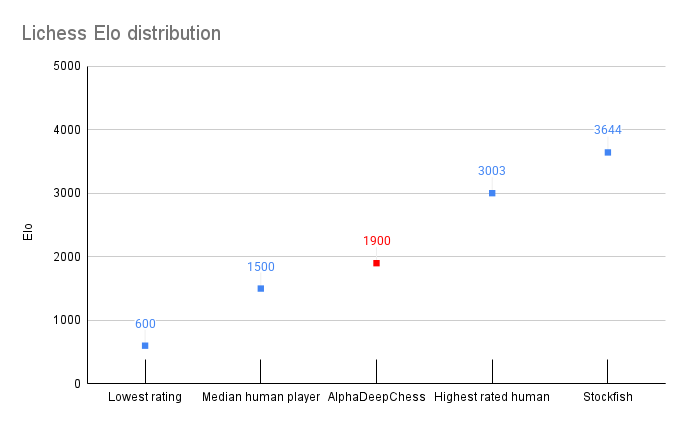
\includegraphics[width=0.95\linewidth]{Imagenes/eloDistribution.png}
    \caption{\textit{Lichess} Elo distribution as of May 2025~\cite{LichessEloDistribution}.}\label{fig:eloDistribution}
\end{figure}
\chapter{Conclusions and Future Work}
\label{cap:conclusiones}

\dots

The next steps to be implemented would be the application of neural networks (NNUE\footnote{\url{https://en.wikipedia.org/wiki/Efficiently_updatable_neural_network}}) which, although intended for CPUs, could be thought of as a streamlined evaluation with GPUs as performed by Leela Chess Zero.

%%%%%%%%%%%%%%%%%%%%%%%%%%%%%%%%%%%%%%%%%%%%%%%%%%%%%%%%%%%%%%%%%%%%%%%%%%%
% Si el TFG se escribe en inglés, comentar las siguientes líneas 
% porque no es necesario incluir nuevamente las Conclusiones en inglés
%\begin{otherlanguage}{english}
%\chapter*{Introduction}
\label{cap:introduction}
\addcontentsline{toc}{chapter}{Introduction}

Introduction to the subject area. This chapter contains the translation of Chapter \ref{cap:introduccion}.










%\chapter*{Conclusions and Future Work}
\label{cap:conclusions}
\addcontentsline{toc}{chapter}{Conclusions and Future Work}

Conclusions and future lines of work. This chapter contains the translation of Chapter \ref{cap:conclusiones}.

TODO

%\end{otherlanguage}
%%%%%%%%%%%%%%%%%%%%%%%%%%%%%%%%%%%%%%%%%%%%%%%%%%%%%%%%%%%%%%%%%%%%%%%%%%%

\chapter{Personal contributions}\label{cap:contribucionesPersonales}

The following section details the individual contributions made by each team member, Juan and Yi, throughout the development of the \textit{AlphaDeepChess} project. Each contribution is listed to provide transparency regarding the division of work, highlight specific areas of responsibility, and acknowledge the expertise and effort invested by each author.

\section*{Juan Girón Herranz}

\begin{itemize}[itemsep=1pt]

    \item Contributed to the alpha-beta pruning algorithm. Taking part in the research and implementation of the iterative deepening and the algorithm core.

    \item Designed and implemented the bitboard-based move generator, then optimized the calculation of the slider pieces moves with magic bitboards technique and the PEXT hardware instruction. Additionally, integrated of the move generator in the search algorithm.

    \item Involved in the implementation of the board data structure, with emphasis on the game state bit field design.

    \item Design and developed the move data structure, which was also optimized as a bit field to reduce space consumption.    

    \item Designed and implemented the auxiliary data structures for rows, columns, diagonals, and directions. These structures played a key role in simplifying and optimizing bitboard masking operations, enabling more efficient move generation and attack pattern calculations.
    
    \item Researched, designed and implemented the transposition table using Zobrist hashing, with total integration in the alpha-beta search.

    \item Introduced MVV-LVA (Most Valuable Victim, Least Valuable Aggressor) in the implementation, then research and enhanced the algorithm with killer-move heuristics.

    \item Researched and developed the quiescence search enhancement to avoid the horizon effect in the alpha-beta pruning.

    \item Developed and tested the search with the late move reductions technique.

    \item Developed the tampering evaluation, adjusting the weight for the middlegame and endgame evaluations, also contributed to optimizations in the implementation for king safety and piece mobility.

    \item Created the algorithm to detect threefold repetition using the game's position history and its implementation in the search.

    \item Implemented part of the UCI command parsing and communication for engine integration.

    \item Conducted multiple 100-game matches using \textit{Cutechess} between engine versions to measure the impact of each optimization.

    \item Created hundreds of unit tests, which have been a fundamental part of finding bugs and ensuring code quality. This includes Perft testing of the move generator, a standard technique that counts all possible legal positions up to a certain depth to ensure the correctness of move generation in the chess engine.

    \item Contributed to the development of a helper GUI in Python to facilitate interactive testing of the engine, with support for the UCI protocol.    

    \item Used Linux's \texttt{perf} tool, analyzed the CPU overhead of the different parts of the chess engine.

    \item Compiled and deployed the engine on a Raspberry Pi 5, configuring it as a \textit{Lichess} bot. Running under limited hardware resources, the engine achieved competitive ELO ratings while demonstrating our code's efficiency and portability.

\end{itemize}

\section*{Yi Wang Qiu}

\begin{itemize}[itemsep=1pt]
    \item Responsible for the architectural design and full implementation of the alpha-beta pruning algorithm, established as the foundational search technique of the engine. This algorithm was enhanced through iterative refinement, such as aspiration windows, and theoretical benchmarking, enabling effective traversal of the game tree while significantly reducing the computational overhead associated with brute-force minimax strategies.

    \item Developed an optimized multithreaded search version incorporating the Young Brothers Wait Concept (YBWC), a parallelization paradigm specifically tailored for game tree evaluation.

    \item Engineered the parsing and command interpretation system compliant with the Universal Chess Interface (UCI) protocol. This subsystem ensures seamless bidirectional communication between the chess engine and external graphical user interfaces, testing suites, and benchmarking frameworks.

    \item Designed and implemented the core engine abstractions, \texttt{Square} and \texttt{Board} classes, which supports the representation and manipulation of chess positions. These classes encapsulate critical logic such as coordinate translation or position translation from FEN, piece tracking, castling rights, and \textit{en passant} possibilities, all integrated with a bitboard backend. This design allows high-level readability while preserving low-level computational performance.

    \item Constructed the internal board representation model using 64-bit bitboards. This representation supports highly efficient binary operations such as masking, shifting, and logical conjunctions to simulate piece movement and board updates.

    \item Developed a modular and extensible evaluation system capable of quantifying chess positions through multiple heuristic lenses. The implemented strategies range from basic material balance (expressed in centipawns) to more sophisticated models that incorporate positional features such as game phase, piece activity, mobility scoring, and king vulnerability or safety. These heuristics were designed to be dynamically weighted depending on the stage of the game (opening, middlegame, or endgame).

    \item Integrated and calibrated the precomputed positional data structures, including piece-square tables to accelerate the static evaluation of positions.

    \item Designed and authored a suite of automated Python scripts for orchestrating engine versus engine tournaments and performance benchmarking using \textit{Cutechess CLI}. These scripts included configurable match parameters like search time, depth of search, number of games, book of openings or initial positions. They were essential in enabling the reproducibility of experiments, comparison of successive versions of the engine, and quantification of the impact of algorithmic refinements.

    \item Established a robust continuous integration and delivery (CI/CD) pipeline using GitHub Actions. This infrastructure automated the build, deployment, and testing stages of the engine. Used the above Python scripts to automate the tournaments in an independent machine to avoid wasting time and computation capacity while still developing.

    \item Contributed to the frontend layer of the project by prototyping a graphical user interface (GUI) in Python, designed to allow interactive execution of the engine in a visual environment. The GUI included subprocess communication features, move display, and optional positional evaluations. Although later iterations focused on headless execution, this interface was key during early debugging and demonstration phases.

    \item Authored detailed and structured online documentation describing the engine's internal architecture, modular hierarchy, function-level responsibilities, and usage guidelines. The documentation was designed not only as an educational resource for future contributors, but also as a formal exposition of the system's logic for academic evaluation purposes like this exact document. It includes illustrative diagrams or graphs, code references, and configuration examples to support transparency and reproducibility.
\end{itemize}


%
% Bibliografía
%
% Si el TFM se escribe en inglés, editar TeXiS/TeXiS_bib para cambiar el
% estilo de las referencias
%---------------------------------------------------------------------
%
%                      configBibliografia.tex
%
%---------------------------------------------------------------------
%
% bibliografia.tex
% Copyright 2009 Marco Antonio Gomez-Martin, Pedro Pablo Gomez-Martin
%
% This file belongs to the TeXiS manual, a LaTeX template for writting
% Thesis and other documents. The complete last TeXiS package can
% be obtained from http://gaia.fdi.ucm.es/projects/texis/
%
% Although the TeXiS template itself is distributed under the 
% conditions of the LaTeX Project Public License
% (http://www.latex-project.org/lppl.txt), the manual content
% uses the CC-BY-SA license that stays that you are free:
%
%    - to share & to copy, distribute and transmit the work
%    - to remix and to adapt the work
%
% under the following conditions:
%
%    - Attribution: you must attribute the work in the manner
%      specified by the author or licensor (but not in any way that
%      suggests that they endorse you or your use of the work).
%    - Share Alike: if you alter, transform, or build upon this
%      work, you may distribute the resulting work only under the
%      same, similar or a compatible license.
%
% The complete license is available in
% http://creativecommons.org/licenses/by-sa/3.0/legalcode
%
%---------------------------------------------------------------------
%
% Fichero  que  configura  los  parámetros  de  la  generación  de  la
% bibliografía.  Existen dos  parámetros configurables:  los ficheros
% .bib que se utilizan y la frase célebre que aparece justo antes de la
% primera referencia.
%
%---------------------------------------------------------------------


%%%%%%%%%%%%%%%%%%%%%%%%%%%%%%%%%%%%%%%%%%%%%%%%%%%%%%%%%%%%%%%%%%%%%%
% Definición de los ficheros .bib utilizados:
% \setBibFiles{<lista ficheros sin extension, separados por comas>}
% Nota:
% Es IMPORTANTE que los ficheros estén en la misma línea que
% el comando \setBibFiles. Si se desea utilizar varias líneas,
% terminarlas con una apertura de comentario.
%%%%%%%%%%%%%%%%%%%%%%%%%%%%%%%%%%%%%%%%%%%%%%%%%%%%%%%%%%%%%%%%%%%%%%
\setBibFiles{%
biblio%
}

%%%%%%%%%%%%%%%%%%%%%%%%%%%%%%%%%%%%%%%%%%%%%%%%%%%%%%%%%%%%%%%%%%%%%%
% Definición de la frase célebre para el capítulo de la
% bibliografía. Dentro normalmente se querrá hacer uso del entorno
% \begin{FraseCelebre}, que contendrá a su vez otros dos entornos,
% un \begin{Frase} y un \begin{Fuente}.
%
% Nota:
% Si no se quiere cita, se puede eliminar su definición (en la
% macro setCitaBibliografia{} ).
%%%%%%%%%%%%%%%%%%%%%%%%%%%%%%%%%%%%%%%%%%%%%%%%%%%%%%%%%%%%%%%%%%%%%%
\setCitaBibliografia{
\begin{FraseCelebre}
\begin{Frase}
  Y así, del mucho leer y del poco dormir, se le secó el celebro de
  manera que vino a perder el juicio.\\ 
  \textcolor{red}{(modificar en Cascaras$\backslash$bibliografia.tex)}
\end{Frase}
\begin{Fuente}
  Miguel de Cervantes Saavedra
\end{Fuente}
\end{FraseCelebre}
}

%%
%% Creamos la bibliografia
%%
\makeBib

% Variable local para emacs, para  que encuentre el fichero maestro de
% compilación y funcionen mejor algunas teclas rápidas de AucTeX

%%%
%%% Local Variables:
%%% mode: latex
%%% TeX-master: "../Tesis.tex"
%%% End:



% Apéndices
% \appendix
% \chapter{Título del Apéndice A}
\label{Appendix:Key1}

Los apéndices son secciones al final del documento en las que se agrega texto con el objetivo de ampliar los contenidos del documento principal.
% \chapter{Título del Apéndice B}
\label{Appendix:Key2}

Se pueden añadir los apéndices que se consideren oportunos.
%\include{Apendices/appendixC}
%\include{...}
%\include{...}
%\include{...}
\backmatter



%
% Índice de palabras
%

% Sólo  la   generamos  si  está   declarada  \generaindice.  Consulta
% TeXiS.sty para más información.

% En realidad, el soporte para la generación de índices de palabras
% en TeXiS no está documentada en el manual, porque no ha sido usada
% "en producción". Por tanto, el fichero que genera el índice
% *no* se incluye aquí (está comentado). Consulta la documentación
% en TeXiS_pream.tex para más información.
\ifx\generaindice\undefined
\else
%%---------------------------------------------------------------------
%
%                        TeXiS_indice.tex
%
%---------------------------------------------------------------------
%
% TeXiS_indice.tex
% Copyright 2009 Marco Antonio Gomez-Martin, Pedro Pablo Gomez-Martin
%
% This file belongs to TeXiS, a LaTeX template for writting
% Thesis and other documents. The complete last TeXiS package can
% be obtained from http://gaia.fdi.ucm.es/projects/texis/
%
% This work may be distributed and/or modified under the
% conditions of the LaTeX Project Public License, either version 1.3
% of this license or (at your option) any later version.
% The latest version of this license is in
%   http://www.latex-project.org/lppl.txt
% and version 1.3 or later is part of all distributions of LaTeX
% version 2005/12/01 or later.
%
% This work has the LPPL maintenance status `maintained'.
% 
% The Current Maintainers of this work are Marco Antonio Gomez-Martin
% and Pedro Pablo Gomez-Martin
%
%---------------------------------------------------------------------
%
% Contiene  los  comandos  para  generar  el índice  de  palabras  del
% documento.
%
%---------------------------------------------------------------------
%
% NOTA IMPORTANTE: el  soporte en TeXiS para el  índice de palabras es
% embrionario, y  de hecho  ni siquiera se  describe en el  manual. Se
% proporciona  una infraestructura  básica (sin  terminar)  para ello,
% pero  no ha  sido usada  "en producción".  De hecho,  a pesar  de la
% existencia de  este fichero, *no* se incluye  en Tesis.tex. Consulta
% la documentación en TeXiS_pream.tex para más información.
%
%---------------------------------------------------------------------


% Si se  va a generar  la tabla de  contenidos (el índice  habitual) y
% también vamos a  generar el índice de palabras  (ambas decisiones se
% toman en  función de  la definición  o no de  un par  de constantes,
% puedes consultar modo.tex para más información), entonces metemos en
% la tabla de contenidos una  entrada para marcar la página donde está
% el índice de palabras.

\ifx\generatoc\undefined
\else
   \addcontentsline{toc}{chapter}{\indexname}
\fi


% Generamos el índice
\printindex

% Variable local para emacs, para  que encuentre el fichero maestro de
% compilación y funcionen mejor algunas teclas rápidas de AucTeX

%%%
%%% Local Variables:
%%% mode: latex
%%% TeX-master: "./tesis.tex"
%%% End:

\fi

%
% Lista de acrónimos
%

% Sólo  lo  generamos  si  está declarada  \generaacronimos.  Consulta
% TeXiS.sty para más información.


\ifx\generaacronimos\undefined
\else
%---------------------------------------------------------------------
%
%                        TeXiS_acron.tex
%
%---------------------------------------------------------------------
%
% TeXiS_acron.tex
% Copyright 2009 Marco Antonio Gomez-Martin, Pedro Pablo Gomez-Martin
%
% This file belongs to TeXiS, a LaTeX template for writting
% Thesis and other documents. The complete last TeXiS package can
% be obtained from http://gaia.fdi.ucm.es/projects/texis/
%
% This work may be distributed and/or modified under the
% conditions of the LaTeX Project Public License, either version 1.3
% of this license or (at your option) any later version.
% The latest version of this license is in
%   http://www.latex-project.org/lppl.txt
% and version 1.3 or later is part of all distributions of LaTeX
% version 2005/12/01 or later.
%
% This work has the LPPL maintenance status `maintained'.
% 
% The Current Maintainers of this work are Marco Antonio Gomez-Martin
% and Pedro Pablo Gomez-Martin
%
%---------------------------------------------------------------------
%
% Contiene  los  comandos  para  generar  el listado de acrónimos
% documento.
%
%---------------------------------------------------------------------
%
% NOTA IMPORTANTE:  para que la  generación de acrónimos  funcione, al
% menos  debe  existir  un  acrónimo   en  el  documento.  Si  no,  la
% compilación  del   fichero  LaTeX  falla  con   un  error  "extraño"
% (indicando  que  quizá  falte  un \item).   Consulta  el  comentario
% referente al paquete glosstex en TeXiS_pream.tex.
%
%---------------------------------------------------------------------


% Redefinimos a español  el título de la lista  de acrónimos (Babel no
% lo hace por nosotros esta vez)

\def\listacronymname{Lista de acrónimos}

% Para el glosario:
% \def\glosarryname{Glosario}

% Si se  va a generar  la tabla de  contenidos (el índice  habitual) y
% también vamos a  generar la lista de acrónimos  (ambas decisiones se
% toman en  función de  la definición  o no de  un par  de constantes,
% puedes consultar config.tex  para más información), entonces metemos
% en la  tabla de contenidos una  entrada para marcar  la página donde
% está el índice de palabras.

\ifx\generatoc\undefined
\else
   \addcontentsline{toc}{chapter}{\listacronymname}
\fi


% Generamos la lista de acrónimos (en realidad el índice asociado a la
% lista "acr" de GlossTeX)

\printglosstex(acr)

% Variable local para emacs, para  que encuentre el fichero maestro de
% compilación y funcionen mejor algunas teclas rápidas de AucTeX

%%%
%%% Local Variables:
%%% mode: latex
%%% TeX-master: "../Tesis.tex"
%%% End:

\fi

%
% Final
%
% %---------------------------------------------------------------------
%
%                      fin.tex
%
%---------------------------------------------------------------------
%
% fin.tex
% Copyright 2009 Marco Antonio Gomez-Martin, Pedro Pablo Gomez-Martin
%
% This file belongs to the TeXiS manual, a LaTeX template for writting
% Thesis and other documents. The complete last TeXiS package can
% be obtained from http://gaia.fdi.ucm.es/projects/texis/
%
% Although the TeXiS template itself is distributed under the 
% conditions of the LaTeX Project Public License
% (http://www.latex-project.org/lppl.txt), the manual content
% uses the CC-BY-SA license that stays that you are free:
%
%    - to share & to copy, distribute and transmit the work
%    - to remix and to adapt the work
%
% under the following conditions:
%
%    - Attribution: you must attribute the work in the manner
%      specified by the author or licensor (but not in any way that
%      suggests that they endorse you or your use of the work).
%    - Share Alike: if you alter, transform, or build upon this
%      work, you may distribute the resulting work only under the
%      same, similar or a compatible license.
%
% The complete license is available in
% http://creativecommons.org/licenses/by-sa/3.0/legalcode
%
%---------------------------------------------------------------------
%
% Contiene la última página
%
%---------------------------------------------------------------------


% Ponemos el marcador en el PDF
\ifpdf
   \pdfbookmark{Fin}{fin}
\fi

\thispagestyle{empty}\mbox{}

Este texto se puede encontrar en el fichero Cascaras/fin.tex. Si deseas eliminarlo, basta con comentar la línea correspondiente al final del fichero TFGTeXiS.tex.

\vspace*{4cm}

\small

\hfill \emph{--¿Qué te parece desto, Sancho? -- Dijo Don Quijote --}

\hfill \emph{Bien podrán los encantadores quitarme la ventura,}

\hfill \emph{pero el esfuerzo y el ánimo, será imposible.}

\hfill 

\hfill \emph{Segunda parte del Ingenioso Caballero} 

\hfill \emph{Don Quijote de la Mancha}

\hfill \emph{Miguel de Cervantes}

\vfill%space*{4cm}

\hfill \emph{--Buena está -- dijo Sancho --; fírmela vuestra merced.}

\hfill \emph{--No es menester firmarla -- dijo Don Quijote--,}

\hfill \emph{sino solamente poner mi rúbrica.}

\hfill 

\hfill \emph{Primera parte del Ingenioso Caballero} 

\hfill \emph{Don Quijote de la Mancha}

\hfill \emph{Miguel de Cervantes}


\newpage
\thispagestyle{empty}\mbox{}

\newpage

% Variable local para emacs, para  que encuentre el fichero maestro de
% compilación y funcionen mejor algunas teclas rápidas de AucTeX

%%%
%%% Local Variables:
%%% mode: latex
%%% TeX-master: "../Tesis.tex"
%%% End:

%\end{otherlanguage}
\end{document}
